% Options for packages loaded elsewhere
\PassOptionsToPackage{unicode}{hyperref}
\PassOptionsToPackage{hyphens}{url}
%
\documentclass[
  11pt,
]{article}
\usepackage{amsmath,amssymb}
\usepackage{lmodern}
\usepackage{iftex}
\ifPDFTeX
  \usepackage[T1]{fontenc}
  \usepackage[utf8]{inputenc}
  \usepackage{textcomp} % provide euro and other symbols
\else % if luatex or xetex
  \usepackage{unicode-math}
  \defaultfontfeatures{Scale=MatchLowercase}
  \defaultfontfeatures[\rmfamily]{Ligatures=TeX,Scale=1}
  \setmainfont[]{Times New Roman}
\fi
% Use upquote if available, for straight quotes in verbatim environments
\IfFileExists{upquote.sty}{\usepackage{upquote}}{}
\IfFileExists{microtype.sty}{% use microtype if available
  \usepackage[]{microtype}
  \UseMicrotypeSet[protrusion]{basicmath} % disable protrusion for tt fonts
}{}
\makeatletter
\@ifundefined{KOMAClassName}{% if non-KOMA class
  \IfFileExists{parskip.sty}{%
    \usepackage{parskip}
  }{% else
    \setlength{\parindent}{0pt}
    \setlength{\parskip}{6pt plus 2pt minus 1pt}}
}{% if KOMA class
  \KOMAoptions{parskip=half}}
\makeatother
\usepackage{xcolor}
\usepackage[margin=1.0in]{geometry}
\usepackage{color}
\usepackage{fancyvrb}
\newcommand{\VerbBar}{|}
\newcommand{\VERB}{\Verb[commandchars=\\\{\}]}
\DefineVerbatimEnvironment{Highlighting}{Verbatim}{commandchars=\\\{\}}
% Add ',fontsize=\small' for more characters per line
\usepackage{framed}
\definecolor{shadecolor}{RGB}{248,248,248}
\newenvironment{Shaded}{\begin{snugshade}}{\end{snugshade}}
\newcommand{\AlertTok}[1]{\textcolor[rgb]{0.94,0.16,0.16}{#1}}
\newcommand{\AnnotationTok}[1]{\textcolor[rgb]{0.56,0.35,0.01}{\textbf{\textit{#1}}}}
\newcommand{\AttributeTok}[1]{\textcolor[rgb]{0.77,0.63,0.00}{#1}}
\newcommand{\BaseNTok}[1]{\textcolor[rgb]{0.00,0.00,0.81}{#1}}
\newcommand{\BuiltInTok}[1]{#1}
\newcommand{\CharTok}[1]{\textcolor[rgb]{0.31,0.60,0.02}{#1}}
\newcommand{\CommentTok}[1]{\textcolor[rgb]{0.56,0.35,0.01}{\textit{#1}}}
\newcommand{\CommentVarTok}[1]{\textcolor[rgb]{0.56,0.35,0.01}{\textbf{\textit{#1}}}}
\newcommand{\ConstantTok}[1]{\textcolor[rgb]{0.00,0.00,0.00}{#1}}
\newcommand{\ControlFlowTok}[1]{\textcolor[rgb]{0.13,0.29,0.53}{\textbf{#1}}}
\newcommand{\DataTypeTok}[1]{\textcolor[rgb]{0.13,0.29,0.53}{#1}}
\newcommand{\DecValTok}[1]{\textcolor[rgb]{0.00,0.00,0.81}{#1}}
\newcommand{\DocumentationTok}[1]{\textcolor[rgb]{0.56,0.35,0.01}{\textbf{\textit{#1}}}}
\newcommand{\ErrorTok}[1]{\textcolor[rgb]{0.64,0.00,0.00}{\textbf{#1}}}
\newcommand{\ExtensionTok}[1]{#1}
\newcommand{\FloatTok}[1]{\textcolor[rgb]{0.00,0.00,0.81}{#1}}
\newcommand{\FunctionTok}[1]{\textcolor[rgb]{0.00,0.00,0.00}{#1}}
\newcommand{\ImportTok}[1]{#1}
\newcommand{\InformationTok}[1]{\textcolor[rgb]{0.56,0.35,0.01}{\textbf{\textit{#1}}}}
\newcommand{\KeywordTok}[1]{\textcolor[rgb]{0.13,0.29,0.53}{\textbf{#1}}}
\newcommand{\NormalTok}[1]{#1}
\newcommand{\OperatorTok}[1]{\textcolor[rgb]{0.81,0.36,0.00}{\textbf{#1}}}
\newcommand{\OtherTok}[1]{\textcolor[rgb]{0.56,0.35,0.01}{#1}}
\newcommand{\PreprocessorTok}[1]{\textcolor[rgb]{0.56,0.35,0.01}{\textit{#1}}}
\newcommand{\RegionMarkerTok}[1]{#1}
\newcommand{\SpecialCharTok}[1]{\textcolor[rgb]{0.00,0.00,0.00}{#1}}
\newcommand{\SpecialStringTok}[1]{\textcolor[rgb]{0.31,0.60,0.02}{#1}}
\newcommand{\StringTok}[1]{\textcolor[rgb]{0.31,0.60,0.02}{#1}}
\newcommand{\VariableTok}[1]{\textcolor[rgb]{0.00,0.00,0.00}{#1}}
\newcommand{\VerbatimStringTok}[1]{\textcolor[rgb]{0.31,0.60,0.02}{#1}}
\newcommand{\WarningTok}[1]{\textcolor[rgb]{0.56,0.35,0.01}{\textbf{\textit{#1}}}}
\usepackage{graphicx}
\makeatletter
\def\maxwidth{\ifdim\Gin@nat@width>\linewidth\linewidth\else\Gin@nat@width\fi}
\def\maxheight{\ifdim\Gin@nat@height>\textheight\textheight\else\Gin@nat@height\fi}
\makeatother
% Scale images if necessary, so that they will not overflow the page
% margins by default, and it is still possible to overwrite the defaults
% using explicit options in \includegraphics[width, height, ...]{}
\setkeys{Gin}{width=\maxwidth,height=\maxheight,keepaspectratio}
% Set default figure placement to htbp
\makeatletter
\def\fps@figure{htbp}
\makeatother
\setlength{\emergencystretch}{3em} % prevent overfull lines
\providecommand{\tightlist}{%
  \setlength{\itemsep}{0pt}\setlength{\parskip}{0pt}}
\setcounter{secnumdepth}{5}
\newlength{\cslhangindent}
\setlength{\cslhangindent}{1.5em}
\newlength{\csllabelwidth}
\setlength{\csllabelwidth}{3em}
\newlength{\cslentryspacingunit} % times entry-spacing
\setlength{\cslentryspacingunit}{\parskip}
\newenvironment{CSLReferences}[2] % #1 hanging-ident, #2 entry spacing
 {% don't indent paragraphs
  \setlength{\parindent}{0pt}
  % turn on hanging indent if param 1 is 1
  \ifodd #1
  \let\oldpar\par
  \def\par{\hangindent=\cslhangindent\oldpar}
  \fi
  % set entry spacing
  \setlength{\parskip}{#2\cslentryspacingunit}
 }%
 {}
\usepackage{calc}
\newcommand{\CSLBlock}[1]{#1\hfill\break}
\newcommand{\CSLLeftMargin}[1]{\parbox[t]{\csllabelwidth}{#1}}
\newcommand{\CSLRightInline}[1]{\parbox[t]{\linewidth - \csllabelwidth}{#1}\break}
\newcommand{\CSLIndent}[1]{\hspace{\cslhangindent}#1}
\newcommand{\bcenter}{\begin{center}}
\newcommand{\ecenter}{\end{center}}
\newcommand{\btitlepage}{\begin{titlepage}}
\newcommand{\etitlepage}{\end{titlepage}}
\usepackage{setspace}\onehalfspacing
\usepackage{booktabs}
\usepackage[font=small,labelfont=bf]{caption}
\usepackage{booktabs}
\usepackage{longtable}
\usepackage{array}
\usepackage{multirow}
\usepackage{wrapfig}
\usepackage{float}
\usepackage{colortbl}
\usepackage{pdflscape}
\usepackage{tabu}
\usepackage{threeparttable}
\usepackage{threeparttablex}
\usepackage[normalem]{ulem}
\usepackage{makecell}
\usepackage{xcolor}
\ifLuaTeX
  \usepackage{selnolig}  % disable illegal ligatures
\fi
\IfFileExists{bookmark.sty}{\usepackage{bookmark}}{\usepackage{hyperref}}
\IfFileExists{xurl.sty}{\usepackage{xurl}}{} % add URL line breaks if available
\urlstyle{same} % disable monospaced font for URLs
\hypersetup{
  hidelinks,
  pdfcreator={LaTeX via pandoc}}

\author{}
\date{\vspace{-2.5em}}

\begin{document}

\begin{titlepage}

\begin{center}

\vspace*{30mm}

Candidate number: 49045

\vspace*{5mm}

\hypertarget{replication-of-hansen-2015-punishment-and-deterrence-evidence-from-drunk-driving}{%
\section*{Replication of Hansen (2015) Punishment and Deterrence:
Evidence from Drunk
Driving}\label{replication-of-hansen-2015-punishment-and-deterrence-evidence-from-drunk-driving}}
\addcontentsline{toc}{section}{Replication of Hansen (2015) Punishment
and Deterrence: Evidence from Drunk Driving}

\vspace*{5mm}

Word count: 2739

\vspace*{30mm}

Submitted as the summative assessment for\\

PB4A7: Quantitative Applications for Behavioural Science 2022

\end{center}

\end{titlepage}

\newpage

In the study \emph{Punishment and Deterrence: Evidence from Drunk
Driving} (Hansen, 2015), Hansen investigated the effect of punishments
and sanctions on reducing repeat drunk driving. The study used a
regression discontinuity design (RDD), utilising the administrative data
from 1995 to 2011 of the state of Washington, U.S., where two thresholds
of blood alcohol content (BAC) are used to determine the status of
driving under the influence (DUI). Specifically, a driver with a BAC
over 0.08 is considered a case of DUI and will be punished via measures
such as fines, jail time, and driving license suspension. One with a BAC
over 0.15 is considered a case of aggravated DUI, to which more severe
punishments and sanctions are applied.

To address the above research question, using the RDD with the BAC as
the running variable is justified for several reasons. First, the BAC
has clear-cut numeric thresholds for determining the severity of
punishments. Second, whether a driver has a BAC level just above or
below the thresholds is justifiably assumed to be completely random.
Third, neither drivers nor police can manipulate the BAC measure.
Applying RDD, Hansen hypothesised that receiving harsher punishments and
sanctions at both thresholds would reduce offenders' future recidivism
of DUI. This hypothesis was supported by the findings of the study.

The present study aims to replicate the findings from Hansen (2015)
using the RDD applied to the data provided by the course instructor. It
will only be focused on the effect of receiving punishments on
recidivism at the 0.08 BAC threshold. The paper proceeds as follows.
Section 1 describes the data and the econometrics method, and discusses
the assumptions of applying the RDD. Section 2 presents the main
results, and Section 3 discusses the results as well as critiques and
extensions to the original study. Section 4 concludes.

\hypertarget{data-methods-and-assumptions}{%
\section{Data, Methods, and
Assumptions}\label{data-methods-and-assumptions}}

\hypertarget{data}{%
\subsection{Data}\label{data}}

The data on which the present study is based is provided by the class
instructor. It documents the BAC level of each driver, the time when it
was measured, and whether it was measured at a traffic accident. The
data also contains information on drivers' recidivism, gender, race, and
age.

\hypertarget{assumptions-of-the-rdd}{%
\subsection{Assumptions of the RDD}\label{assumptions-of-the-rdd}}

Several assumptions are required for the RDD to give accurate estimates
(See Appendix B for a discussion on manipulation). One of these is that
the running variable should not contain non-random heaping (Barreca et
al., 2016). This means that BAC should not be much more likely to take
certain values than others, which can bias the estimates if occurring at
the threshold. Based on the histogram of the BAC as a continuous
variable (Figure \ref{fig:bac_hist_continuous}), this assumption seems
to be violated. Curiously, when the BAC is plotted as a discrete
variable, non-random heaping disappears (Figure
\ref{fig:bac_hist_discrete}).

\begin{figure}[H]
  \centering
  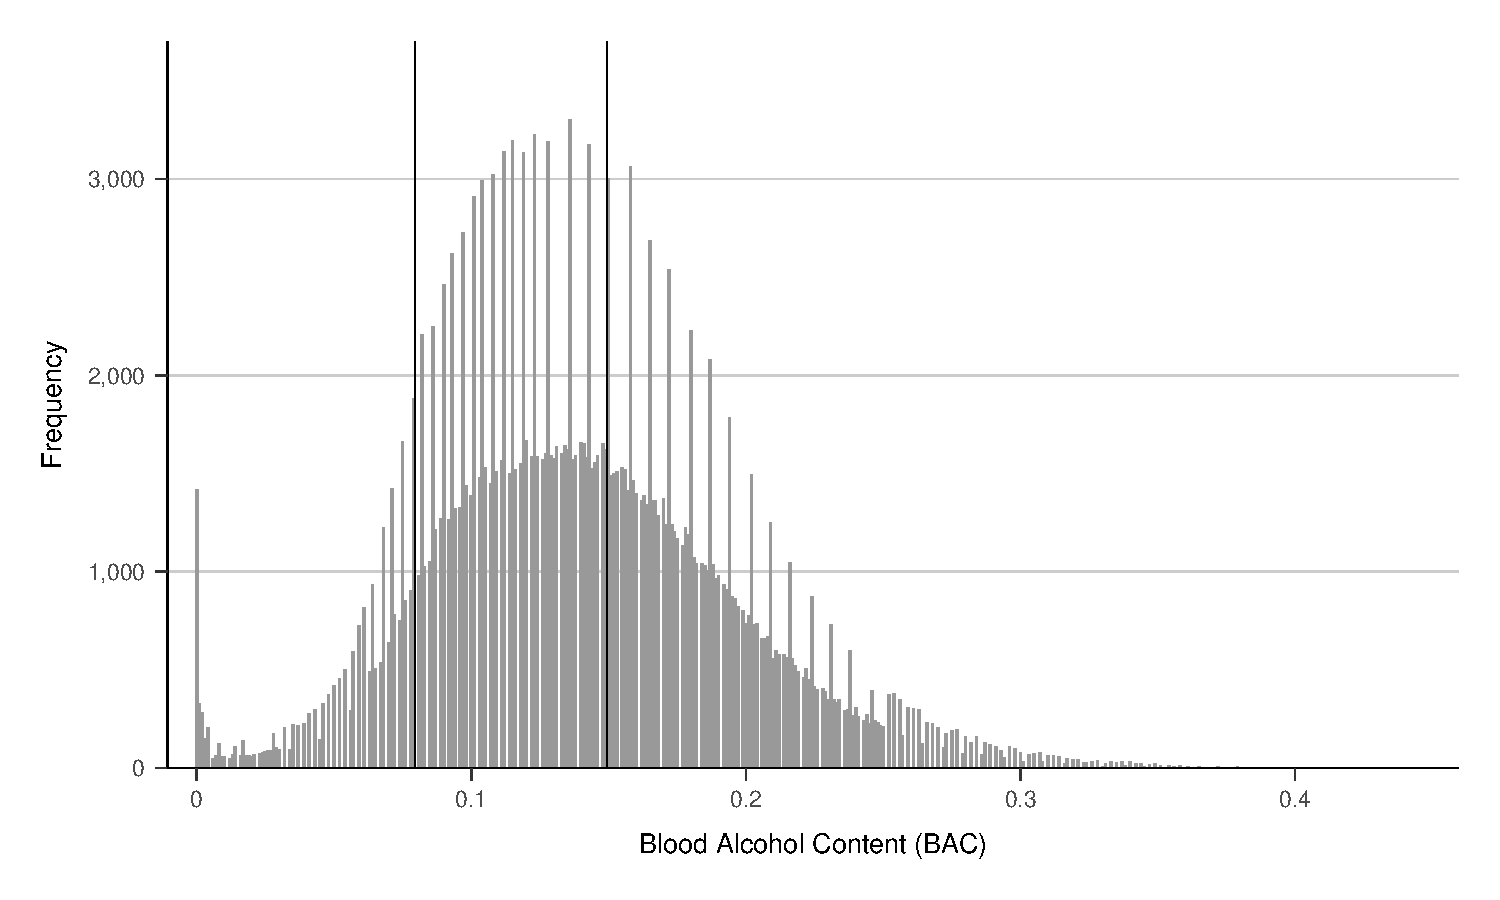
\includegraphics[width=0.9\columnwidth]{../figures/bac_histogram_continuous.pdf}
  \caption{\textbf{Histogram of blood alcohol content as a continuous variable.} The blood alcohol content is plotted as a continuous variable with a bin width of 0.001, the precision used on the breathalysers. The y-axis represents the frequency of observations in each bin. The vertical black lines represent the two thresholds at 0.08 and 0.15.}
  \label{fig:bac_hist_continuous}
\end{figure}

A closer inspection of the data suggests that this is probably due to
the lack of precision in the BAC in the current data. Many BAC values
deviate by a very small amount from the values that are supposed to be
given by the breathalysers (i.e., precise to three digits after the
decimal point). For some bins, the measured BAC value at the left
boundary deviate upwards and the value at the right boundary deviating
downwards. Such bins will contain a larger number of observations than
their neighbours and thus lead to heaping (See Appendix C for a detailed
discussion based on simulations).

\begin{figure}[H]
  \centering
  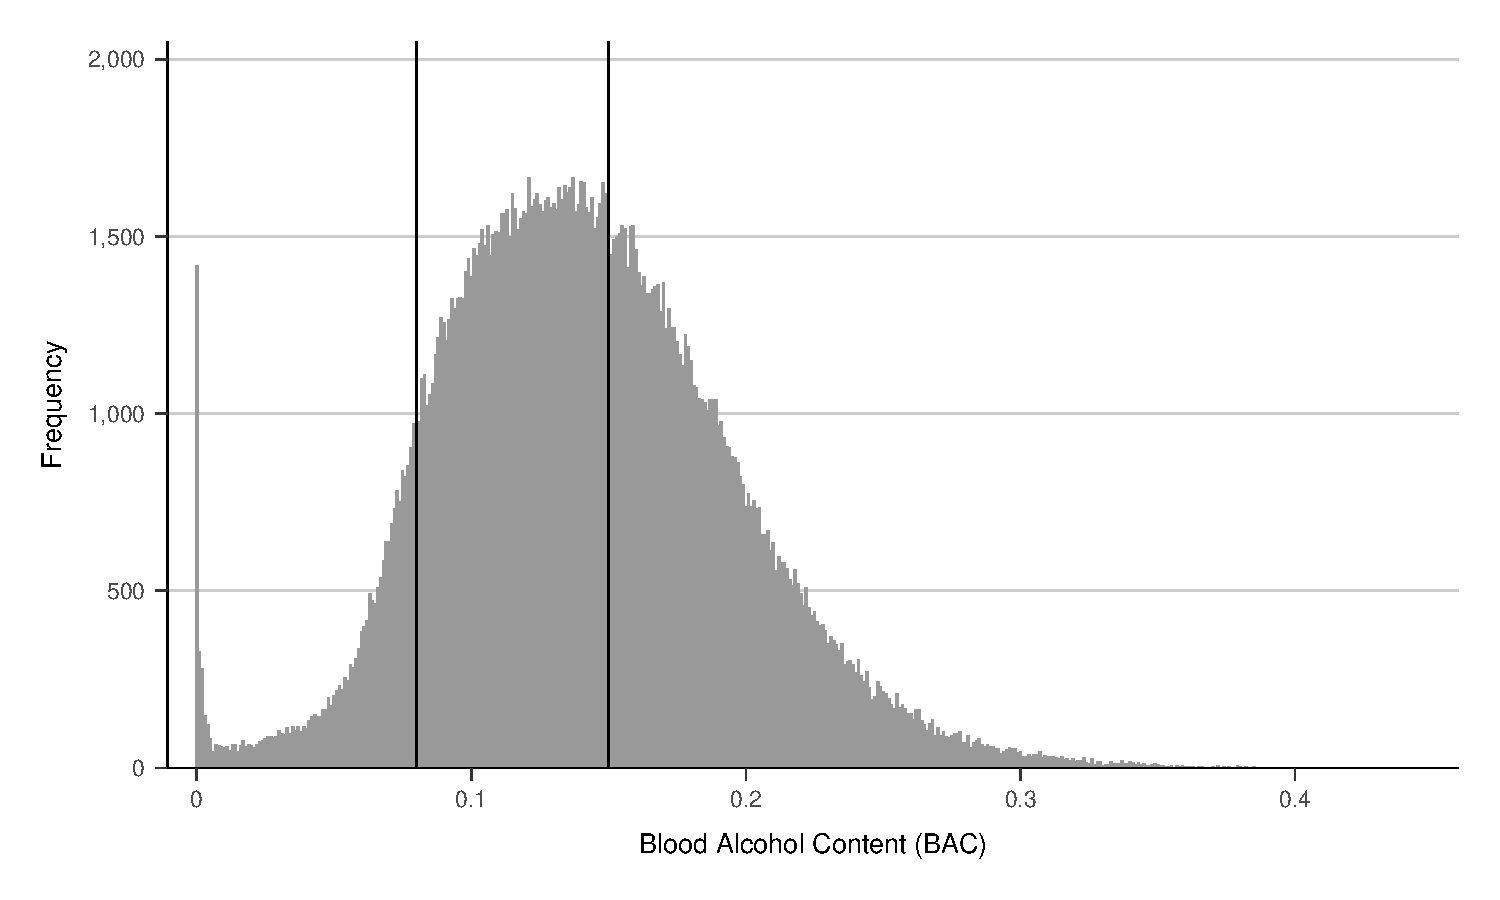
\includegraphics[width=0.9\columnwidth]{../figures/bac_histogram_discrete.pdf}
  \caption{\textbf{Histogram of blood alcohol content as a discrete variable.} The blood alcohol content is plotted as a discrete variable with a bin width of 0.001, the precision used on the breathalysers. The y-axis represents the frequency of observations in each bin. The vertical black lines represent the two thresholds at 0.08 and 0.15.}
  \label{fig:bac_hist_discrete}
\end{figure}

\hypertarget{the-model-and-control-variables}{%
\subsection{The model and control
variables}\label{the-model-and-control-variables}}

Similar to the original study (Hansen, 2015), the present study utilises
a local linear regression model with a rectangular kernel weight
function to estimate the effect of receiving punishments at the
threshold on recidivism. For sensitivity analyses, the models are
re-estimated using second-order polynomials or a triangle kernel
function (See Appendix B for model details).

To determine the control variables, I run preliminary analyses on the
effect of receiving punishments at the threshold on four predetermined
characteristics, including three demographic variables (gender, race,
and age) and the BAC test being conducted in a traffic accident. The
analyses use the same local linear regression model as the main
analyses, with a bandwidth of 0.05 and a rectangular kernel weight
function. As Table \ref{tab:covariate} shows, I fail to reject any of
the null hypotheses that predetermined characteristics remained the same
at the threshold. This indicates that gender, race, age, and the BAC
test being conducted in a traffic accident, on average, were not
different between people who did not receive punishments and those who
received punishments at the threshold. According to Calonico et al.
(2019), I will include the four predetermined characteristics in
regression discontinuity models to improve the precision of the
estimation.

\begingroup
\renewcommand{\arraystretch}{1.3}

\begin{table}

\caption{Regression Discontinuity Estimates of the Effect of Receiving Punishments at the 0.08 BAC Threshold on Predetermined Characteristics}
\label{tab:covariate}
\centering
\begin{threeparttable}
\begin{tabular}[t]{l>{\centering\arraybackslash}p{5em}>{\centering\arraybackslash}p{5em}>{\centering\arraybackslash}p{5em}>{\centering\arraybackslash}p{5em}}
\toprule
  & Male & White & Age & Accident\\
\midrule
\textit{DUI} & 0.006 & 0.006 & –0.141 & –0.003\\
 & (0.006) & (0.005) & (0.164) & (0.004)\\
Mean & 0.784 & 0.846 & 0.085 & 33.99\\
Num. of Obs. & 89,967 & 89,967 & 89,967 & 89,967\\
\bottomrule
\end{tabular}
\begin{tablenotes}
\small
\item \textit{Note.} Regression discontinuity based estimates of the effect of receiving punishments at the 0.08 BAC threshold on four predetermined characteristics. All models use a bandwidth of 0.05 and a rectangular kernel weight function. Counterfactual predictions of mean recidivism is calculated at the 0.079 BAC threshold. Heteroscedasticity-robust standard errors are in parentheses.
\item $^{*}\, p<0.1$, $^{**}\, p<0.05$, $^{***}\, p<0.01$.
\end{tablenotes}
\end{threeparttable}
\end{table}

\endgroup

\hypertarget{results}{%
\section{Results}\label{results}}

\hypertarget{the-effect-of-receiving-punishments-on-recidivism}{%
\subsection{The Effect of Receiving Punishments on
Recidivism}\label{the-effect-of-receiving-punishments-on-recidivism}}

Table \ref{tab:main} reports the estimated effect of receiving
punishments at the threshold on recidivism. The local linear regression
model with a rectangular kernel function gives the estimate that
receiving punishments at the 0.08 BAC threshold decreases recidivism by
2.4 percentage points, which is statistically significant at the level
of 0.01. The local second-order polynomial with a rectangular kernel
function gives an estimate of a decrease by 1.4 percentage points, which
is statistically significant at the level of 0.05. These estimates are
consistent across both bandwidths and across models with different types
of kernel functions.

\begingroup
\renewcommand{\arraystretch}{1.1}

\begin{table}

\caption{Regression Discontinuity Estimates of the Effect of Receiving Punishments at the 0.08 BAC Threshold on Recidivism}
\label{tab:main}
\centering
\begin{threeparttable}
\begin{tabular}[t]{l>{\centering\arraybackslash}p{8em}>{\centering\arraybackslash}p{8em}>{\centering\arraybackslash}p{8em}>{\centering\arraybackslash}p{8em}}
\toprule
\multicolumn{1}{c}{ } & \multicolumn{2}{c}{Rectangular kernel} & \multicolumn{2}{c}{Triangular kernel} \\
\cmidrule(l{3pt}r{3pt}){2-3} \cmidrule(l{3pt}r{3pt}){4-5}
  & Linear & Quadratic & Linear & Quadratic\\
\midrule
\multicolumn{5}{l}{\textit{A. DUI $\in$ [0.03, 0.13]}} \\
\textit{DUI} & –0.024*** & –0.014** & –0.020*** & –0.014**\\
 & (0.004) & (0.006) & (0.005) & (0.006)\\
Mean & 0.104 & 0.099 & 0.100 & 0.099\\
Controls & Yes & Yes & Yes & Yes\\
Num. of Obs. & 89,967 & 89,967 & 89,967 & 89,967\\
\addlinespace
\multicolumn{5}{l}{\textit{B. DUI $\in$ [0.055, 0.105]}} \\
\textit{DUI} & –0.021*** & –0.014* & –0.018*** & –0.016*\\
 & (0.006) & (0.008) & (0.006) & (0.009)\\
Mean & 0.101 & 0.098 & 0.101 & 0.100\\
Controls & Yes & Yes & Yes & Yes\\
Num. of Obs. & 46,957 & 46,957 & 46,957 & 46,957\\
\bottomrule
\end{tabular}
\begin{tablenotes}
\small
\item \textit{Note.} Regression discontinuity based estimates of the effect of receiving punishments at the 0.08 BAC threshold on recidivism. Panel A presents estimates based on a 0.05 bandwidth, and Panel B presents estimates based on a 0.025 bandwidth. The table includes results from both linear and quadratic models, with either a rectangular or a triangular kernel weight function. Controls include individuals' gender, race, age, and an indicator of whether the BAC test was conducted in a traffic accident. Counterfactual predictions of mean recidivism are calculated at the 0.079 BAC threshold and mean age of the respective populations, averaging over individuals' gender and race, as well as over whether the BAC testing was conducted in an accident. Heteroscedasticity-robust standard errors are in parentheses.
\item $^{*}\, p<0.1$, $^{**}\, p<0.05$, $^{***}\, p<0.01$.
\end{tablenotes}
\end{threeparttable}
\end{table}

\endgroup

Figure \ref{fig:rdplot} plots means of observed recidivism in bins and
predicted recidivism based on linear regression models or second-order
polynomials within the interval \(BAC \in [0.06, 0.11]\). Panel A and B
and Panel C and D use different methods for binning observations and
representing confidence intervals to ensure the robustness of the visual
evidence (See the figure caption) (Calonico, Cattaneo, et al., 2015a).
All panels show an apparent drop in recidivism at the BAC threshold of
0.08. This visually indicates that there is an effect of receiving
punishments at the threshold in decreasing recidivism.

\begin{figure}[H]
  \centering
  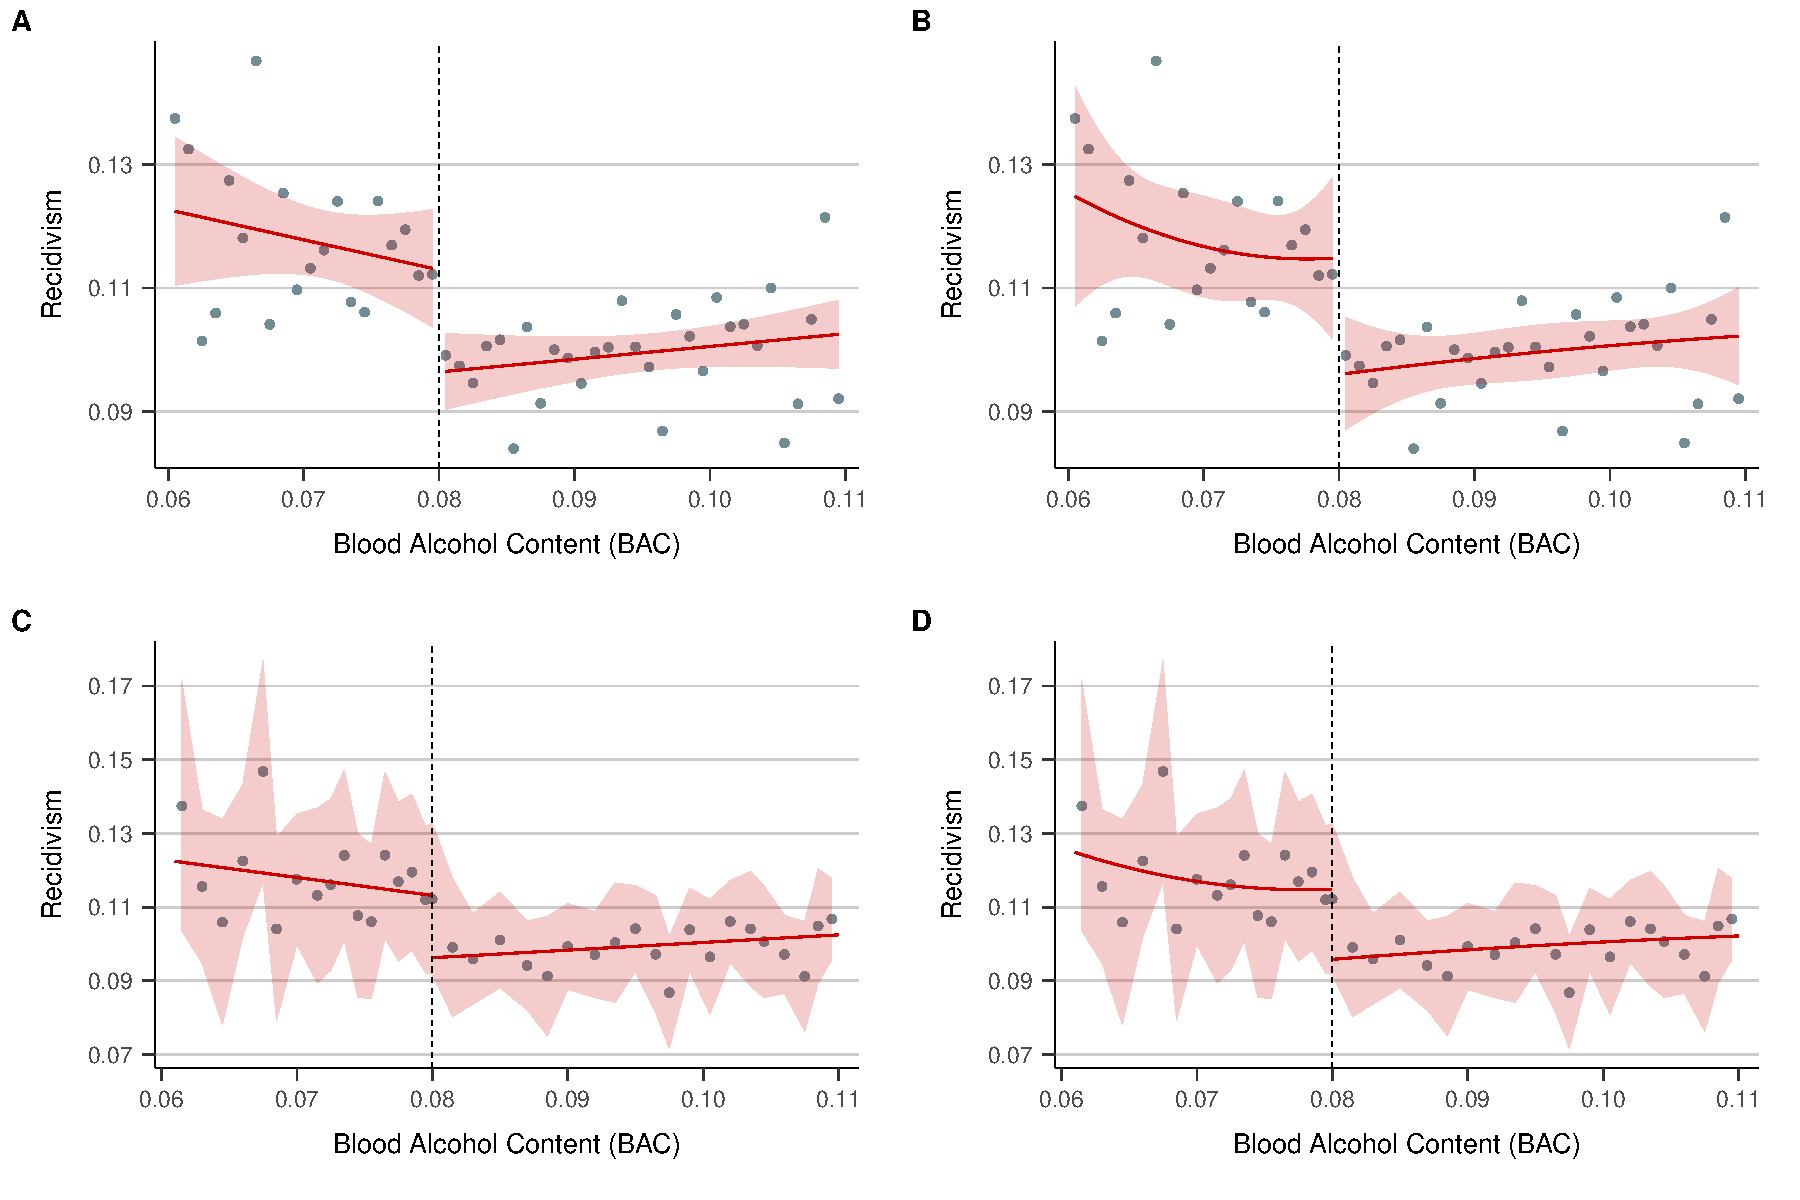
\includegraphics[width=1\columnwidth]{../figures/combined.pdf}
  \caption{\textbf{Regression Discontinuity Plot of the Effect of Receiving Punishments at the 0.08 BAC Threshold on Recidivism.} Plot of means of recidivism in bins and predicted recidivism using simple regression models. In plotting the binned means (the grey points), Panel A and B choose the number of bins on each side of the threshold using the formula $min\{\sqrt{n}, 10 \times \frac{\ln{n}}{\ln{10}}\}$, while Panel C and D choose the number using quantile spaced binning (Calonico, Cattaneo, et al., 2015a). For the confidence intervals (the shaded areas in red), Panel A and B plot the 95\% confidence interval of the regression models, while Panel C and D plot the 95\% confidence interval of each bin. For the regression models (the red lines), Panel A and C plot the best fitted linear models, while Panel B and D plot the best fitted second-order polynomials. All panels plot the data within the interval $BAC \in [0.06, 0.11]$. The vertical dashed lines represent the BAC threshold at 0.08.}
  \label{fig:rdplot}
\end{figure}

\hypertarget{robustness}{%
\subsection{Robustness}\label{robustness}}

Since there seems to be non-random heaping in the current data (Figure
\ref{fig:bac_hist_continuous}), this section will use donut hole
regression discontinuity models to investigate the robustness of the
results. The donut hole approach entirely drops the observations near
the threshold before fitting an RD model. Under appropriate assumptions,
it is effective in preventing a heap just at the threshold from biasing
the estimates (Barreca et al., 2016).

For the present study, I drop the observations in the interval
\(BAC \in [0.079, 0.081]\), and re-estimate local linear and quadratic
models with either a rectangular or a triangular kernel weight function.
It is worth stressing that local polynomials are especially important
for donut hole models. This is because the donut hole approach gets rid
of the very observations on which the estimates of local average effects
rely upon. The estimates given by donut hole models are essentially
based on models' extrapolation over the region of the donut hole (Dowd,
2021) and may be especially sensitive to the assumptions about the
underlying functional form. Using polynomials with different orders can
ensure the robustness of the results over different functional
assumptions (See Appendix C for a detailed discussion based on
simulations).

The results from donut hole models are presented in Table
\ref{tab:donut}. According to the local linear regression model with a
rectangular kernel function, receiving punishments at the threshold
decreases recidivism by 2.6 percentage points and is statistically
significant at the level of 0.01. According to the local second-order
polynomial with a rectangular kernel function, the decrease is 1.4
percentage points and is statistically significant at the level of 0.1.
These estimates are consistent across both bandwidths and across models
with different types of kernel functions, except for not being
statistically significant in quadratic models estimated with a narrower
bandwidth. Therefore, the results given by donut hole models are
essentially similar with those given by ordinary RDD models.

\begingroup
\renewcommand{\arraystretch}{1.1}

\begin{table}

\caption{Donut Regression Discontinuity Estimates of the Effect of Receiving Punishments at the 0.08 BAC Threshold on Recidivism}
\label{tab:donut}
\centering
\begin{threeparttable}
\begin{tabular}[t]{l>{\centering\arraybackslash}p{8em}>{\centering\arraybackslash}p{8em}>{\centering\arraybackslash}p{8em}>{\centering\arraybackslash}p{8em}}
\toprule
\multicolumn{1}{c}{ } & \multicolumn{2}{c}{Rectangular kernel} & \multicolumn{2}{c}{Triangular kernel} \\
\cmidrule(l{3pt}r{3pt}){2-3} \cmidrule(l{3pt}r{3pt}){4-5}
  & Linear & Quadratic & Linear & Quadratic\\
\midrule
\multicolumn{5}{l}{\textit{A. DUI $\in$ [0.03, 0.13]}} \\
\textit{DUI} & –0.026*** & –0.014* & –0.022*** & –0.018**\\
 & (0.005) & (0.007) & (0.005) & (0.006)\\
Mean & 0.105 & 0.099 & 0.102 & 0.101\\
Controls & Yes & Yes & Yes & Yes\\
Num. of Obs. & 88,085 & 88,085 & 88,085 & 88,085\\
\addlinespace
\multicolumn{5}{l}{\textit{B. DUI $\in$ [0.055, 0.105]}} \\
\textit{DUI} & –0.022*** & –0.015 & –0.020*** & –0.020\\
 & (0.007) & (0.011) & (0.007) & (0.012)\\
Mean & 0.103 & 0.099 & 0.103 & 0.104\\
Controls & Yes & Yes & Yes & Yes\\
Num. of Obs. & 45,075 & 45,075 & 45,075 & 45,075\\
\bottomrule
\end{tabular}
\begin{tablenotes}
\small
\item \textit{Note.} Regression discontinuity based estimates of the effect of receiving punishments at the 0.08 BAC threshold on recidivism after dropping observations in the interval [0.079, 0.081]. Panel A presents estimates based on a 0.05 bandwidth, and Panel B presents estimates based on a 0.025 bandwidth. The table includes results from both linear and quadratic models, with either a rectangular or a triangular kernel weight function. Controls include individuals' gender, race, age, and an indicator of whether the BAC test was conducted in a traffic accident. Counterfactual predictions of mean recidivism are calculated at the 0.079 BAC threshold and mean age of the respective populations, averaging over individuals' gender and race, as well as over whether the BAC testing was conducted in an accident. Heteroscedasticity-robust standard errors are in parentheses.
\item $^{*}\, p<0.1$, $^{**}\, p<0.05$, $^{***}\, p<0.01$.
\end{tablenotes}
\end{threeparttable}
\end{table}

\endgroup

\hypertarget{discussion-critique-and-extension}{%
\section{Discussion, Critique and
Extension}\label{discussion-critique-and-extension}}

Using a regression discontinuity design, the present study aims to
replicate the findings of Hansen (2015) about the effect of punishments
and sanctions on reducing repeat drunk driving. Specifically, the
present study focuses on testing whether receiving punishments at the
0.08 Blood Alcohol Content (BAC) threshold reduces future recidivism of
drunk driving. The findings based on local linear regression models show
that receiving punishments at the threshold reduces recidivism by up to
2.4 percentage points
\footnote{The average estimated effect is 2.1 percentage points. The average estimate is calculated over models based on different bandwidths and with different kernel functions, assuming equal weights of estimates.}.
Sensitivity analyses based on local second-order polynomials show that
receiving punishments at the threshold reduces recidivism by up to 1.6
percentage points
\footnote{The average estimated effect is 1.5 percentage points.}. These
estimates are consistent with those given by the models that take into
account non-random heaping in the data, establishing the robustness of
the results.

\hypertarget{strengths-of-the-original-study}{%
\subsection{Strengths of the original
study}\label{strengths-of-the-original-study}}

The findings of the present study successfully replicate the main
results of Hansen (2015), which gives an estimated decrease caused by
receiving punishments of up to 2 percentage points at the 0.08 BAC
threshold. The success of the replication demonstrates the validity of
the methodology and results of the original study. Hansen (2015) also
presents related results that the present study, due to its scope and
the limitation of the data available, does not replicate. As a part of
the strengths of the original study, these findings either establish the
robustness of the main results under different assumptions or reveal the
heterogeneity of the effect of receiving punishments.

In terms of the robustness of the main results, the original study
estimates regression discontinuity models using polynomials up to the
third order, three types of kernel functions, and based on a series of
bandwidths that extend beyond 0.05 and 0.025. The results show that the
point estimates are relatively consistent, only except for those given
by the local second-order polynomials and those estimated based on very
small bandwidths.

The heterogeneity of the effects of punishments include the effects
among different populations and the effect on different types of
recidivism. First of all, the original study separates analyses for
drivers with and without prior drunk driving experience, in addition to
running regression models on the entire population of drivers. This
allows the original study to find that the effect of receiving
punishments at the threshold is more pronounced among drivers with
previous drunk driving experience. Second, the original study conducts a
detailed analyses of the effect of receiving punishments on three types
of recidivism, refusal of taking a BAC test, and the likelihood of being
stopped by a police. It finds that receiving punishments decreases the
likelihood of being stopped as well as recidivism of all kinds. Both
results reveal the heterogeneous nature of the effect of receiving
punishments on recidivism.

\hypertarget{suggested-improvements-and-extentions}{%
\subsection{Suggested improvements and
extentions}\label{suggested-improvements-and-extentions}}

Despite multiple strengths of the original study, it can still be
improved in several aspects. First, the primary bandwidths used in the
original study (0.05 and 0.025) seem to be arbitrary choices of the
researcher. Bandwidth choice can be improved by using data-driven
methods with a predetermined principle. For example, Mean Squared Error
(MSE) optimal bandwidth is an available method and has recently been
improved for better inference with a bias correction (Cattaneo \&
Vazquez-Bare, 2017; Imbens \& Kalyanaraman, 2012). Alternatively, one
can choose to use a method that minimises coverage error (CE)
probability when the goal is to construct optimal confidence intervals
for inference (Calonico et al., 2022). Both MSE-optimal and CE-optimal
bandwidths are based on the data and constructed according to an
explicit desideratum, which makes the bandwidth choice more objective
and transparent. Future research can and should make full use of these
methods as they are readily available in packages of mainstream
statistical software (Calonico, Cattaneo, et al., 2015b; Calonico et
al., 2017).

Second, in light of the present study, local second-order polynomials
consistently give lower estimates than linear models. In fact, this is
also the finding of the original study (Appendix Table 5 of Hansen,
2015). This suggests that the estimates of the effect of receiving
punishments at the threshold somewhat depend on the assumptions about
the effect's functional form. Although it is difficult to pin down one
reasonable functional assumption due to the complex nature of the
effect, future research should give equal weights in presenting the
results given by different models. This is especially important for such
an estimand that is closely associated with policy making, since even a
small difference in the estimate can lead to big differences when scaled
up.

Third, the use of simple linear regression models is inadequate when
recidivism, the outcome variable, is a binary variable. In simple words,
this is because of a mathematical inconsistency between the range of the
outcome variable (which can only take the value of 0 and 1) and the
range of a linear regression model (which can take the value of any real
number). Future research can utilise logistic regressions in combination
with the RDD to estimate the effect of punishments on recidivism. This
should not be a difficult task because recent research in econometrics
has developed and programmed such methods based on the multinomial logit
model, together with optimal bandwidth selection and bias correction
techniques (Xu, 2017).

Fourth, the robustness checks using donut hole regression discontinuity
models are limited. Although the original study excluded the possibility
of non-random heaping based on a histogram, the treatment of the
variable (i.e., continuous vs.~discrete) of which is unclear, non-random
heaping may exist in the original data in light of the present study. If
this were the case, the donut hole approach could potentially still give
biased estimates. This is because non-random heaping outside the
dropping window can bias the estimation (Barreca et al., 2016). Future
studies can adopt a solution suggested by previous research, that is, to
separate the analyses for non-heaped data and heap points (if any).
Unbiased estimates can be derived by taking a population-weighted
average of the two estimates based on the respective sample sizes
(Barreca et al., 2016).

Finally, the external and internal validity of the study can be improved
in future extensions. To improve the external validity of the
estimation, one can use data from regions other than the state of
Washington. This is to establish that punishments are universally
effective in reducing repeat drunk driving across regions and the effect
is not caused by some other factors specific to the state of Washington.
The internal validity of the causal relation can be improved by
conducting a longitudinal field experiment. One can choose a region
where laws criminalizing DUI are not yet enforced, and carry out an
experiment by manipulating the magnitude of the punishments received by
drivers if found driving under the influence. Drivers with a BAC level
just below a chosen threshold are randomly assigned to receive lighter
punishments than those with a BAC level just above the threshold. This
method can theoretically provide stronger evidence for the causal
relation between receiving punishments and recidivism. However, there
are also challenges to such designs. For example, it is hard to prevent
spillover effects. Drivers may find out punishments vary among
individuals, and the consequence of such an effect is essentially
unpredictable. Ethically speaking, it also invites debates on how such
an experiment can adhere to the principle of transparency. Due to the
scope of this paper, I will leave these challenges to be addressed by
future research.

\hypertarget{conclusion}{%
\section{Conclusion}\label{conclusion}}

The present study successfully replicates the main results of the study
\emph{Punishment and Deterrence: Evidence from Drunk Driving} (Hansen,
2015) about the effect of punishments and sanctions on reducing repeat
drunk driving using a regression discontinuity design. Specifically, I
find that receiving punishments at the 0.08 BAC threshold reduces
recidivism by up to 2.4 percentage points according to local linear
regression models, and the decrease is up to 1.6 percentage points
according to local second-order polynomials. These results provide
evidence for the validity of the original study. The original study also
conducts additional analyses to establish the robustness of the results
and reveal heterogeneity of the effects. Despite these strengths, the
original study can be improved in aspects such as bandwidth selection,
the selection of appropriate models and robustness checks, the
presentation of the results, as well as internal and external validity.

\newpage

\hypertarget{references}{%
\section*{References}\label{references}}
\addcontentsline{toc}{section}{References}

\hypertarget{refs}{}
\begin{CSLReferences}{1}{0}
\leavevmode\vadjust pre{\hypertarget{ref-barreca_heaping-induced_2016}{}}%
Barreca, A. I., Lindo, J. M., \& Waddell, G. R. (2016). Heaping-induced
bias in regression-discontinuity designs. \emph{Economic Inquiry},
\emph{54}(1), 268--293. \url{https://doi.org/10.1111/ecin.12225}

\leavevmode\vadjust pre{\hypertarget{ref-calonico_coverage_2022}{}}%
Calonico, S., Cattaneo, M. D., \& Farrell, M. H. (2022). Coverage error
optimal confidence intervals for local polynomial regression.
\emph{Bernoulli}, \emph{28}(4). \url{https://doi.org/10.3150/21-BEJ1445}

\leavevmode\vadjust pre{\hypertarget{ref-calonico_regression_2019}{}}%
Calonico, S., Cattaneo, M. D., Farrell, M. H., \& Titiunik, R. (2019).
Regression discontinuity designs using covariates. \emph{The Review of
Economics and Statistics}, \emph{101}(3), 442--451.
\url{https://doi.org/10.1162/rest_a_00760}

\leavevmode\vadjust pre{\hypertarget{ref-calonico_rdrobust_2017}{}}%
Calonico, S., Cattaneo, M. D., Farrell, M. H., \& Titiunik, R. (2017).
{rdrobust}: Software for regression-discontinuity designs. \emph{The
Stata Journal}, \emph{17}(2), 372--404.
https://doi.org/\url{https://doi.org/10.1177/1536867X1701700208}

\leavevmode\vadjust pre{\hypertarget{ref-calonico_optimal_2015}{}}%
Calonico, S., Cattaneo, M. D., \& Titiunik, R. (2015a). Optimal
data-driven regression discontinuity plots. \emph{Journal of the
American Statistical Association}, \emph{110}(512), 1753--1769.
\url{https://doi.org/10.1080/01621459.2015.1017578}

\leavevmode\vadjust pre{\hypertarget{ref-calonico_rdrobust_2015}{}}%
Calonico, S., Cattaneo, M., D., \& Titiunik, R. (2015b). {rdrobust}: An
{R} package for robust nonparametric inference in
regression-discontinuity designs. \emph{The R Journal}, \emph{7}(1), 38.
\url{https://doi.org/10.32614/RJ-2015-004}

\leavevmode\vadjust pre{\hypertarget{ref-cattaneo_simple_2020}{}}%
Cattaneo, M. D., Jansson, M., \& Ma, X. (2020). Simple local polynomial
density estimators. \emph{Journal of the American Statistical
Association}, \emph{115}(531), 1449--1455.
\url{https://doi.org/10.1080/01621459.2019.1635480}

\leavevmode\vadjust pre{\hypertarget{ref-cattaneo_choice_2017}{}}%
Cattaneo, M. D., \& Vazquez-Bare, G. (2017). The choice of neighborhood
in regression discontinuity designs. \emph{Observational Studies},
\emph{3}(2), 134--146.
https://doi.org/\url{https://doi.org/10.1353/obs.2017.0002}

\leavevmode\vadjust pre{\hypertarget{ref-dowd_donuts_2021}{}}%
Dowd, C. (2021). \emph{Donuts and distant {CATEs}: Derivative bounds for
{RD} extrapolation} (No. 3641913).
\url{https://doi.org/10.2139/ssrn.3641913}

\leavevmode\vadjust pre{\hypertarget{ref-hansen_punishment_2015}{}}%
Hansen, B. (2015). Punishment and deterrence: Evidence from drunk
driving. \emph{American Economic Review}, \emph{105}(4), 1581--1617.
\url{https://doi.org/10.1257/aer.20130189}

\leavevmode\vadjust pre{\hypertarget{ref-imbens_optimal_2012}{}}%
Imbens, G., \& Kalyanaraman, K. (2012). Optimal bandwidth choice for the
regression discontinuity estimator. \emph{The Review of Economic
Studies}, \emph{79}(3), 933--959.
https://doi.org/\url{https://doi.org/10.1093/restud/rdr043}

\leavevmode\vadjust pre{\hypertarget{ref-xu_regression_2017}{}}%
Xu, K.-L. (2017). Regression discontinuity with categorical outcomes.
\emph{Journal of Econometrics}, \emph{201}(1), 1--18.
\url{https://doi.org/10.1016/j.jeconom.2017.07.004}

\end{CSLReferences}

\newpage

\hypertarget{appendix-a-analysis-code}{%
\section*{Appendix A: Analysis Code}\label{appendix-a-analysis-code}}
\addcontentsline{toc}{section}{Appendix A: Analysis Code}

This appendix presents the code associated with the assignment
questions. A full list of analysis code is stored in the Github
repository (link masked for the anonymity of the report).

\begin{enumerate}
\def\labelenumi{\arabic{enumi}.}
\tightlist
\item
  Create the variables for Driving Under the Influence, and quadratic
  term for Blood alcohol level and produce two histograms of BAC1 (one
  as a discrete variable, one as a continuous). Explain the differences
  of the histograms.
\end{enumerate}

\begin{Shaded}
\begin{Highlighting}[]
\CommentTok{\# load libraries}
\FunctionTok{library}\NormalTok{(tidyverse);}\FunctionTok{library}\NormalTok{(haven);}\FunctionTok{library}\NormalTok{(here)}
\FunctionTok{library}\NormalTok{(rdrobust);}\FunctionTok{library}\NormalTok{(wesanderson)}

\CommentTok{\# input data}
\NormalTok{bac\_data }\OtherTok{\textless{}{-}}
  \FunctionTok{here}\NormalTok{(}\StringTok{"summative/data/hansen\_dwi.dta"}\NormalTok{) }\SpecialCharTok{\%\textgreater{}\%} \CommentTok{\# locate the data}
  \FunctionTok{read\_dta}\NormalTok{() }\SpecialCharTok{\%\textgreater{}\%} \CommentTok{\# read the dta file}
  \CommentTok{\# code variables}
  \FunctionTok{mutate}\NormalTok{(}
    \CommentTok{\# code into drive under influence (dui) = 1 if bac1 \textgreater{}= 0.08}
    \AttributeTok{dui =} \FunctionTok{ifelse}\NormalTok{(bac1 }\SpecialCharTok{\textgreater{}=} \FloatTok{0.08}\NormalTok{, }\DecValTok{1}\NormalTok{, }\DecValTok{0}\NormalTok{),}
    \CommentTok{\# create a centered bac1 variable}
    \AttributeTok{bac1\_ctd =}\NormalTok{ bac1 }\SpecialCharTok{{-}} \FloatTok{0.08}\NormalTok{,}
    \CommentTok{\# create a quadratic term for both bac1 and bac1\_ctd}
    \AttributeTok{bac1\_sq =}\NormalTok{ bac1}\SpecialCharTok{\^{}}\DecValTok{2}\NormalTok{,}
    \AttributeTok{bac1\_ctd\_sq =}\NormalTok{ bac1\_ctd}\SpecialCharTok{\^{}}\DecValTok{2}\NormalTok{,}
    \CommentTok{\# create donut hole for later use}
    \AttributeTok{donut =} \FunctionTok{ifelse}\NormalTok{(}\FunctionTok{abs}\NormalTok{(bac1\_ctd) }\SpecialCharTok{\textless{}=} \FloatTok{0.001}\NormalTok{, }\DecValTok{1}\NormalTok{, }\DecValTok{0}\NormalTok{)}
\NormalTok{    )}

\CommentTok{\# create the histogram treating BAC as a discrete variable}
\CommentTok{\# equivalent to stata function histogram bac1, discrete width(0.001)}
\NormalTok{bac\_data }\SpecialCharTok{\%\textgreater{}\%}
  \FunctionTok{ggplot}\NormalTok{(}\FunctionTok{aes}\NormalTok{(}\AttributeTok{x =}\NormalTok{ bac1)) }\SpecialCharTok{+}
  \FunctionTok{geom\_histogram}\NormalTok{(}\AttributeTok{binwidth =} \FloatTok{0.001}\NormalTok{, }\AttributeTok{fill =} \StringTok{"grey60"}\NormalTok{, }\AttributeTok{color =} \ConstantTok{NA}\NormalTok{) }\SpecialCharTok{+}
  \FunctionTok{geom\_vline}\NormalTok{(}\AttributeTok{xintercept =} \FloatTok{0.08}\NormalTok{, }\AttributeTok{size =} \FloatTok{0.3}\NormalTok{) }\SpecialCharTok{+}
  \FunctionTok{geom\_vline}\NormalTok{(}\AttributeTok{xintercept =} \FloatTok{0.15}\NormalTok{, }\AttributeTok{size =} \FloatTok{0.3}\NormalTok{) }\SpecialCharTok{+}
  \FunctionTok{scale\_x\_continuous}\NormalTok{(}\AttributeTok{breaks =} \FunctionTok{seq}\NormalTok{(}\DecValTok{0}\NormalTok{, }\FloatTok{0.5}\NormalTok{, }\AttributeTok{by =} \FloatTok{0.1}\NormalTok{),}
                     \AttributeTok{labels =} \FunctionTok{c}\NormalTok{(}\StringTok{"0"}\NormalTok{, }\StringTok{"0.1"}\NormalTok{, }\StringTok{"0.2"}\NormalTok{, }\StringTok{"0.3"}\NormalTok{, }\StringTok{"0.4"}\NormalTok{, }\StringTok{"0.5"}\NormalTok{),}
                     \AttributeTok{expand =} \FunctionTok{c}\NormalTok{(}\DecValTok{0}\NormalTok{, }\FloatTok{0.01}\NormalTok{)) }\SpecialCharTok{+}
  \FunctionTok{scale\_y\_continuous}\NormalTok{(}\AttributeTok{breaks =} \FunctionTok{seq}\NormalTok{(}\DecValTok{0}\NormalTok{, }\DecValTok{2000}\NormalTok{, }\AttributeTok{by =} \DecValTok{500}\NormalTok{),}
                     \AttributeTok{labels =} \FunctionTok{c}\NormalTok{(}\StringTok{"0"}\NormalTok{, }\StringTok{"500"}\NormalTok{, }\StringTok{"1,000"}\NormalTok{, }\StringTok{"1,500"}\NormalTok{, }\StringTok{"2,000"}\NormalTok{),}
                     \AttributeTok{limits =} \FunctionTok{c}\NormalTok{(}\DecValTok{0}\NormalTok{, }\DecValTok{2050}\NormalTok{),}
                     \AttributeTok{expand =} \FunctionTok{c}\NormalTok{(}\DecValTok{0}\NormalTok{, }\DecValTok{0}\NormalTok{)) }\SpecialCharTok{+}
  \FunctionTok{labs}\NormalTok{(}\AttributeTok{x =} \StringTok{"Blood Alcohol Content (BAC)"}\NormalTok{, }\AttributeTok{y =} \StringTok{"Frequency"}\NormalTok{) }\SpecialCharTok{+}
  \FunctionTok{theme\_classic}\NormalTok{() }\SpecialCharTok{+}
  \FunctionTok{theme}\NormalTok{(}
    \AttributeTok{panel.grid =} \FunctionTok{element\_blank}\NormalTok{(),}
    \AttributeTok{panel.grid.major.y =} \FunctionTok{element\_line}\NormalTok{(}\AttributeTok{color =} \StringTok{"grey80"}\NormalTok{, }\AttributeTok{size =} \FloatTok{0.4}\NormalTok{),}
    \AttributeTok{axis.line =} \FunctionTok{element\_line}\NormalTok{(}\AttributeTok{size =} \FloatTok{0.4}\NormalTok{),}
    \AttributeTok{axis.text.y =} \FunctionTok{element\_text}\NormalTok{(}\AttributeTok{size =} \DecValTok{11}\NormalTok{, }\AttributeTok{margin =} \FunctionTok{margin}\NormalTok{(}\DecValTok{0}\NormalTok{, }\DecValTok{5}\NormalTok{, }\DecValTok{0}\NormalTok{, }\DecValTok{0}\NormalTok{)),}
    \AttributeTok{axis.text.x =} \FunctionTok{element\_text}\NormalTok{(}\AttributeTok{size =} \DecValTok{11}\NormalTok{, }\AttributeTok{margin =} \FunctionTok{margin}\NormalTok{(}\DecValTok{5}\NormalTok{, }\DecValTok{0}\NormalTok{, }\DecValTok{0}\NormalTok{, }\DecValTok{0}\NormalTok{)),}
    \AttributeTok{axis.ticks =} \FunctionTok{element\_line}\NormalTok{(}\AttributeTok{size =} \FloatTok{0.4}\NormalTok{),}
    \AttributeTok{axis.ticks.length =} \FunctionTok{unit}\NormalTok{(}\DecValTok{6}\NormalTok{, }\AttributeTok{units =} \StringTok{"pt"}\NormalTok{),}
    \AttributeTok{axis.title.y =} \FunctionTok{element\_text}\NormalTok{(}\AttributeTok{size =} \DecValTok{13}\NormalTok{, }\AttributeTok{margin =} \FunctionTok{margin}\NormalTok{(}\DecValTok{0}\NormalTok{, }\DecValTok{10}\NormalTok{, }\DecValTok{0}\NormalTok{, }\DecValTok{0}\NormalTok{)),}
    \AttributeTok{axis.title.x =} \FunctionTok{element\_text}\NormalTok{(}\AttributeTok{size =} \DecValTok{13}\NormalTok{, }\AttributeTok{margin =} \FunctionTok{margin}\NormalTok{(}\DecValTok{10}\NormalTok{, }\DecValTok{0}\NormalTok{, }\DecValTok{0}\NormalTok{, }\DecValTok{0}\NormalTok{)),}
    \AttributeTok{plot.margin =} \FunctionTok{margin}\NormalTok{(}\DecValTok{20}\NormalTok{, }\DecValTok{20}\NormalTok{, }\DecValTok{20}\NormalTok{, }\DecValTok{20}\NormalTok{)}

\NormalTok{  )}
\end{Highlighting}
\end{Shaded}

\begin{Shaded}
\begin{Highlighting}[]
\CommentTok{\# create the histogram treating BAC as a continuous variable}
\CommentTok{\# equivalent to stata function histogram bac1, width(0.001)}
\NormalTok{bac\_data }\SpecialCharTok{\%\textgreater{}\%}
  \FunctionTok{mutate}\NormalTok{(}\AttributeTok{bac1 =}\NormalTok{ bac1 }\SpecialCharTok{{-}} \FloatTok{0.0005}\NormalTok{) }\SpecialCharTok{\%\textgreater{}\%}
  \FunctionTok{ggplot}\NormalTok{(}\FunctionTok{aes}\NormalTok{(}\AttributeTok{x =}\NormalTok{ bac1)) }\SpecialCharTok{+}
  \FunctionTok{geom\_histogram}\NormalTok{(}\AttributeTok{binwidth =} \FloatTok{0.001}\NormalTok{, }\AttributeTok{fill =} \StringTok{"grey60"}\NormalTok{, }\AttributeTok{color =} \ConstantTok{NA}\NormalTok{) }\SpecialCharTok{+}
  \FunctionTok{geom\_vline}\NormalTok{(}\AttributeTok{xintercept =} \FloatTok{0.08} \SpecialCharTok{{-}} \FloatTok{0.0005}\NormalTok{, }\AttributeTok{size =} \FloatTok{0.3}\NormalTok{) }\SpecialCharTok{+}
  \FunctionTok{geom\_vline}\NormalTok{(}\AttributeTok{xintercept =} \FloatTok{0.15} \SpecialCharTok{{-}} \FloatTok{0.0005}\NormalTok{, }\AttributeTok{size =} \FloatTok{0.3}\NormalTok{) }\SpecialCharTok{+}
  \FunctionTok{scale\_x\_continuous}\NormalTok{(}\AttributeTok{breaks =} \FunctionTok{seq}\NormalTok{(}\DecValTok{0}\NormalTok{, }\FloatTok{0.5}\NormalTok{, }\AttributeTok{by =} \FloatTok{0.1}\NormalTok{),}
                     \AttributeTok{labels =} \FunctionTok{c}\NormalTok{(}\StringTok{"0"}\NormalTok{, }\StringTok{"0.1"}\NormalTok{, }\StringTok{"0.2"}\NormalTok{, }\StringTok{"0.3"}\NormalTok{, }\StringTok{"0.4"}\NormalTok{, }\StringTok{"0.5"}\NormalTok{),}
                     \AttributeTok{expand =} \FunctionTok{c}\NormalTok{(}\DecValTok{0}\NormalTok{, }\FloatTok{0.01}\NormalTok{)) }\SpecialCharTok{+}
  \FunctionTok{scale\_y\_continuous}\NormalTok{(}\AttributeTok{breaks =} \FunctionTok{seq}\NormalTok{(}\DecValTok{0}\NormalTok{, }\DecValTok{3000}\NormalTok{, }\AttributeTok{by =} \DecValTok{1000}\NormalTok{),}
                     \AttributeTok{labels =} \FunctionTok{c}\NormalTok{(}\StringTok{"0"}\NormalTok{, }\StringTok{"1,000"}\NormalTok{, }\StringTok{"2,000"}\NormalTok{, }\StringTok{"3,000"}\NormalTok{),}
                     \AttributeTok{limits =} \FunctionTok{c}\NormalTok{(}\DecValTok{0}\NormalTok{, }\DecValTok{3700}\NormalTok{),}
                     \AttributeTok{expand =} \FunctionTok{c}\NormalTok{(}\DecValTok{0}\NormalTok{, }\DecValTok{0}\NormalTok{)) }\SpecialCharTok{+}
  \FunctionTok{labs}\NormalTok{(}\AttributeTok{x =} \StringTok{"Blood Alcohol Content (BAC)"}\NormalTok{, }\AttributeTok{y =} \StringTok{"Frequency"}\NormalTok{) }\SpecialCharTok{+}
  \FunctionTok{theme\_classic}\NormalTok{() }\SpecialCharTok{+}
  \FunctionTok{theme}\NormalTok{(}
    \AttributeTok{panel.grid =} \FunctionTok{element\_blank}\NormalTok{(),}
    \AttributeTok{panel.grid.major.y =} \FunctionTok{element\_line}\NormalTok{(}\AttributeTok{color =} \StringTok{"grey80"}\NormalTok{, }\AttributeTok{size =} \FloatTok{0.4}\NormalTok{),}
    \AttributeTok{axis.line =} \FunctionTok{element\_line}\NormalTok{(}\AttributeTok{size =} \FloatTok{0.4}\NormalTok{),}
    \AttributeTok{axis.text.y =} \FunctionTok{element\_text}\NormalTok{(}\AttributeTok{size =} \DecValTok{11}\NormalTok{, }\AttributeTok{margin =} \FunctionTok{margin}\NormalTok{(}\DecValTok{0}\NormalTok{, }\DecValTok{5}\NormalTok{, }\DecValTok{0}\NormalTok{, }\DecValTok{0}\NormalTok{)),}
    \AttributeTok{axis.text.x =} \FunctionTok{element\_text}\NormalTok{(}\AttributeTok{size =} \DecValTok{11}\NormalTok{, }\AttributeTok{margin =} \FunctionTok{margin}\NormalTok{(}\DecValTok{5}\NormalTok{, }\DecValTok{0}\NormalTok{, }\DecValTok{0}\NormalTok{, }\DecValTok{0}\NormalTok{)),}
    \AttributeTok{axis.ticks =} \FunctionTok{element\_line}\NormalTok{(}\AttributeTok{size =} \FloatTok{0.4}\NormalTok{),}
    \AttributeTok{axis.ticks.length =} \FunctionTok{unit}\NormalTok{(}\DecValTok{6}\NormalTok{, }\AttributeTok{units =} \StringTok{"pt"}\NormalTok{),}
    \AttributeTok{axis.title.y =} \FunctionTok{element\_text}\NormalTok{(}\AttributeTok{size =} \DecValTok{13}\NormalTok{, }\AttributeTok{margin =} \FunctionTok{margin}\NormalTok{(}\DecValTok{0}\NormalTok{, }\DecValTok{10}\NormalTok{, }\DecValTok{0}\NormalTok{, }\DecValTok{0}\NormalTok{)),}
    \AttributeTok{axis.title.x =} \FunctionTok{element\_text}\NormalTok{(}\AttributeTok{size =} \DecValTok{13}\NormalTok{, }\AttributeTok{margin =} \FunctionTok{margin}\NormalTok{(}\DecValTok{10}\NormalTok{, }\DecValTok{0}\NormalTok{, }\DecValTok{0}\NormalTok{, }\DecValTok{0}\NormalTok{)),}
    \AttributeTok{plot.margin =} \FunctionTok{margin}\NormalTok{(}\DecValTok{20}\NormalTok{, }\DecValTok{20}\NormalTok{, }\DecValTok{20}\NormalTok{, }\DecValTok{20}\NormalTok{)}

\NormalTok{  )}
\end{Highlighting}
\end{Shaded}

\begin{enumerate}
\def\labelenumi{\arabic{enumi}.}
\setcounter{enumi}{1}
\tightlist
\item
  Running regressions on covariates (white, male, age and accident) to
  see if there is a jump in average values for each of these at the
  cutoff and explain the results.
\end{enumerate}

\begin{Shaded}
\begin{Highlighting}[]
\CommentTok{\# load the function to display summary statistics with robust standard errors}
\FunctionTok{source}\NormalTok{(}\FunctionTok{here}\NormalTok{(}\StringTok{"summative/code/summaryR.R"}\NormalTok{))}

\CommentTok{\# get the data within the bandwidth}
\NormalTok{dat\_bandwidth\_0}\FloatTok{.05} \OtherTok{\textless{}{-}}\NormalTok{ bac\_data }\SpecialCharTok{\%\textgreater{}\%} \FunctionTok{filter}\NormalTok{(}\FunctionTok{abs}\NormalTok{(bac1\_ctd) }\SpecialCharTok{\textless{}=} \FloatTok{0.05}\NormalTok{)}

\CommentTok{\# check being white}
\NormalTok{white\_rdd }\OtherTok{\textless{}{-}}\NormalTok{ dat\_bandwidth\_0}\FloatTok{.05} \SpecialCharTok{\%\textgreater{}\%} \FunctionTok{lm}\NormalTok{(white }\SpecialCharTok{\textasciitilde{}}\NormalTok{ dui}\SpecialCharTok{*}\NormalTok{bac1\_ctd, }\AttributeTok{data =}\NormalTok{ .)}
\CommentTok{\# display results with robust SEs}
\FunctionTok{summaryR.lm}\NormalTok{(white\_rdd, }\AttributeTok{type =} \StringTok{"hc1"}\NormalTok{)}

\CommentTok{\# check being male}
\NormalTok{male\_rdd }\OtherTok{\textless{}{-}}\NormalTok{ dat\_bandwidth\_0}\FloatTok{.05} \SpecialCharTok{\%\textgreater{}\%} \FunctionTok{lm}\NormalTok{(male }\SpecialCharTok{\textasciitilde{}}\NormalTok{ dui}\SpecialCharTok{*}\NormalTok{bac1\_ctd, }\AttributeTok{data =}\NormalTok{ .)}
\FunctionTok{summaryR.lm}\NormalTok{(male\_rdd, }\AttributeTok{type =} \StringTok{"hc1"}\NormalTok{)}

\CommentTok{\# check accident}
\NormalTok{accident\_rdd }\OtherTok{\textless{}{-}}\NormalTok{ dat\_bandwidth\_0}\FloatTok{.05} \SpecialCharTok{\%\textgreater{}\%} \FunctionTok{lm}\NormalTok{(acc }\SpecialCharTok{\textasciitilde{}}\NormalTok{ dui}\SpecialCharTok{*}\NormalTok{bac1\_ctd, }\AttributeTok{data =}\NormalTok{ .)}
\FunctionTok{summaryR.lm}\NormalTok{(accident\_rdd, }\AttributeTok{type =} \StringTok{"hc1"}\NormalTok{)}

\CommentTok{\# check age}
\NormalTok{age\_rdd }\OtherTok{\textless{}{-}}\NormalTok{ dat\_bandwidth\_0}\FloatTok{.05} \SpecialCharTok{\%\textgreater{}\%} \FunctionTok{lm}\NormalTok{(aged }\SpecialCharTok{\textasciitilde{}}\NormalTok{ dui}\SpecialCharTok{*}\NormalTok{bac1\_ctd, }\AttributeTok{data =}\NormalTok{ .)}
\FunctionTok{summaryR.lm}\NormalTok{(age\_rdd, }\AttributeTok{type =} \StringTok{"hc1"}\NormalTok{)}
\end{Highlighting}
\end{Shaded}

\begin{enumerate}
\def\labelenumi{\arabic{enumi}.}
\setcounter{enumi}{2}
\tightlist
\item
  Produce main recidivism results of the paper (with our dataset) using
  recidivism as dependent variable as well as with a changed bandwith of
  the RDD to 0.055 to 0.105.
\end{enumerate}

\begin{Shaded}
\begin{Highlighting}[]
\CommentTok{\# linear regression}
\NormalTok{linear\_a }\OtherTok{\textless{}{-}}
\NormalTok{  dat\_bandwidth\_0}\FloatTok{.05} \SpecialCharTok{\%\textgreater{}\%}
  \FunctionTok{lm}\NormalTok{(recidivism }\SpecialCharTok{\textasciitilde{}}\NormalTok{ dui}\SpecialCharTok{*}\NormalTok{bac1\_ctd }\SpecialCharTok{+}\NormalTok{ white }\SpecialCharTok{+}\NormalTok{ male }\SpecialCharTok{+}\NormalTok{ acc }\SpecialCharTok{+}\NormalTok{ aged,}
     \AttributeTok{data =}\NormalTok{ .)}
\FunctionTok{summaryR.lm}\NormalTok{(linear\_a, }\AttributeTok{type =} \StringTok{"hc1"}\NormalTok{)}

\CommentTok{\# quadratic model}
\NormalTok{qua\_a }\OtherTok{\textless{}{-}}
\NormalTok{  dat\_bandwidth\_0}\FloatTok{.05} \SpecialCharTok{\%\textgreater{}\%}
  \FunctionTok{lm}\NormalTok{(recidivism }\SpecialCharTok{\textasciitilde{}}\NormalTok{ dui}\SpecialCharTok{*}\NormalTok{(bac1\_ctd }\SpecialCharTok{+}\NormalTok{ bac1\_ctd\_sq) }\SpecialCharTok{+}\NormalTok{ white }\SpecialCharTok{+}\NormalTok{ male }\SpecialCharTok{+}\NormalTok{ acc }\SpecialCharTok{+}\NormalTok{ aged,}
     \AttributeTok{data =}\NormalTok{ .)}
\FunctionTok{summaryR.lm}\NormalTok{(qua\_a, }\AttributeTok{type =} \StringTok{"hc1"}\NormalTok{)}


\CommentTok{\# get the data within the 0.025 bandwidth}
\NormalTok{dat\_bandwidth\_0}\FloatTok{.025} \OtherTok{\textless{}{-}}\NormalTok{ bac\_data }\SpecialCharTok{\%\textgreater{}\%} \FunctionTok{filter}\NormalTok{(}\FunctionTok{abs}\NormalTok{(bac1\_ctd) }\SpecialCharTok{\textless{}=} \FloatTok{0.025}\NormalTok{)}

\CommentTok{\# linear regression}
\NormalTok{linear\_b }\OtherTok{\textless{}{-}}
\NormalTok{  dat\_bandwidth\_0}\FloatTok{.025} \SpecialCharTok{\%\textgreater{}\%}
  \FunctionTok{lm}\NormalTok{(recidivism }\SpecialCharTok{\textasciitilde{}}\NormalTok{ dui}\SpecialCharTok{*}\NormalTok{bac1\_ctd }\SpecialCharTok{+}\NormalTok{ white }\SpecialCharTok{+}\NormalTok{ male }\SpecialCharTok{+}\NormalTok{ acc }\SpecialCharTok{+}\NormalTok{ aged,}
     \AttributeTok{data =}\NormalTok{ .)}
\FunctionTok{summaryR.lm}\NormalTok{(linear\_b, }\AttributeTok{type =} \StringTok{"hc1"}\NormalTok{)}

\CommentTok{\# quadratic model}
\NormalTok{qua\_b }\OtherTok{\textless{}{-}}
\NormalTok{  dat\_bandwidth\_0}\FloatTok{.025} \SpecialCharTok{\%\textgreater{}\%}
  \FunctionTok{lm}\NormalTok{(recidivism }\SpecialCharTok{\textasciitilde{}}\NormalTok{ dui}\SpecialCharTok{*}\NormalTok{(bac1\_ctd }\SpecialCharTok{+}\NormalTok{ bac1\_ctd\_sq) }\SpecialCharTok{+}\NormalTok{ white }\SpecialCharTok{+}\NormalTok{ male }\SpecialCharTok{+}\NormalTok{ acc }\SpecialCharTok{+}\NormalTok{ aged,}
     \AttributeTok{data =}\NormalTok{ .)}
\FunctionTok{summaryR.lm}\NormalTok{(qua\_b, }\AttributeTok{type =} \StringTok{"hc1"}\NormalTok{)}
\end{Highlighting}
\end{Shaded}

\begin{enumerate}
\def\labelenumi{\arabic{enumi}.}
\setcounter{enumi}{3}
\tightlist
\item
  Replicate Qe by running ``donut hole regressions''. Explain why one
  might need a donut hole regression? How do I run a donut hole
  regression?
\item
  Run local polynomials and explain why local polynomials might be
  needed after a donut hole.
\end{enumerate}

\begin{Shaded}
\begin{Highlighting}[]
\CommentTok{\# linear regression}
\NormalTok{linear\_a\_donut }\OtherTok{\textless{}{-}}
\NormalTok{  dat\_bandwidth\_0}\FloatTok{.05} \SpecialCharTok{\%\textgreater{}\%}
  \FunctionTok{filter}\NormalTok{(donut }\SpecialCharTok{==} \DecValTok{0}\NormalTok{) }\SpecialCharTok{\%\textgreater{}\%}
  \FunctionTok{lm}\NormalTok{(recidivism }\SpecialCharTok{\textasciitilde{}}\NormalTok{ dui}\SpecialCharTok{*}\NormalTok{bac1\_ctd }\SpecialCharTok{+}\NormalTok{ white }\SpecialCharTok{+}\NormalTok{ male }\SpecialCharTok{+}\NormalTok{ acc }\SpecialCharTok{+}\NormalTok{ aged,}
     \AttributeTok{data =}\NormalTok{ .)}
\FunctionTok{summaryR.lm}\NormalTok{(linear\_a\_donut, }\AttributeTok{type =} \StringTok{"hc1"}\NormalTok{)}

\CommentTok{\# narrower bandwidth}
\NormalTok{linear\_b\_donut }\OtherTok{\textless{}{-}}
\NormalTok{  dat\_bandwidth\_0}\FloatTok{.025} \SpecialCharTok{\%\textgreater{}\%}
  \FunctionTok{filter}\NormalTok{(donut }\SpecialCharTok{==} \DecValTok{0}\NormalTok{) }\SpecialCharTok{\%\textgreater{}\%}
  \FunctionTok{lm}\NormalTok{(recidivism }\SpecialCharTok{\textasciitilde{}}\NormalTok{ dui}\SpecialCharTok{*}\NormalTok{bac1\_ctd }\SpecialCharTok{+}\NormalTok{ white }\SpecialCharTok{+}\NormalTok{ male }\SpecialCharTok{+}\NormalTok{ acc }\SpecialCharTok{+}\NormalTok{ aged,}
     \AttributeTok{data =}\NormalTok{ .)}
\FunctionTok{summaryR.lm}\NormalTok{(linear\_b\_donut, }\AttributeTok{type =} \StringTok{"hc1"}\NormalTok{)}

\CommentTok{\# quadratic model}
\NormalTok{qua\_a\_donut }\OtherTok{\textless{}{-}}
\NormalTok{  dat\_bandwidth\_0}\FloatTok{.05} \SpecialCharTok{\%\textgreater{}\%}
  \FunctionTok{filter}\NormalTok{(donut }\SpecialCharTok{==} \DecValTok{0}\NormalTok{) }\SpecialCharTok{\%\textgreater{}\%}
  \FunctionTok{lm}\NormalTok{(recidivism }\SpecialCharTok{\textasciitilde{}}\NormalTok{ dui}\SpecialCharTok{*}\NormalTok{(bac1\_ctd }\SpecialCharTok{+}\NormalTok{ bac1\_ctd\_sq) }\SpecialCharTok{+}\NormalTok{ white }\SpecialCharTok{+}\NormalTok{ male }\SpecialCharTok{+}\NormalTok{ acc }\SpecialCharTok{+}\NormalTok{ aged,}
     \AttributeTok{data =}\NormalTok{ .)}
\FunctionTok{summaryR.lm}\NormalTok{(qua\_a\_donut, }\AttributeTok{type =} \StringTok{"hc1"}\NormalTok{)}

\CommentTok{\# narrower bandwidth}
\NormalTok{qua\_b\_donut }\OtherTok{\textless{}{-}}
\NormalTok{  dat\_bandwidth\_0}\FloatTok{.025} \SpecialCharTok{\%\textgreater{}\%}
  \FunctionTok{filter}\NormalTok{(donut }\SpecialCharTok{==} \DecValTok{0}\NormalTok{) }\SpecialCharTok{\%\textgreater{}\%}
  \FunctionTok{lm}\NormalTok{(recidivism }\SpecialCharTok{\textasciitilde{}}\NormalTok{ dui}\SpecialCharTok{*}\NormalTok{(bac1\_ctd }\SpecialCharTok{+}\NormalTok{ bac1\_ctd\_sq) }\SpecialCharTok{+}\NormalTok{ white }\SpecialCharTok{+}\NormalTok{ male }\SpecialCharTok{+}\NormalTok{ acc }\SpecialCharTok{+}\NormalTok{ aged,}
     \AttributeTok{data =}\NormalTok{ .)}
\FunctionTok{summaryR.lm}\NormalTok{(qua\_b\_donut, }\AttributeTok{type =} \StringTok{"hc1"}\NormalTok{)}
\end{Highlighting}
\end{Shaded}

\begin{enumerate}
\def\labelenumi{\arabic{enumi}.}
\setcounter{enumi}{5}
\tightlist
\item
  Produce an RDplot and a cmogram with bandwidths of 0.060 \& 0.11.
  Explain what the respective graphs show.
\end{enumerate}

\begin{Shaded}
\begin{Highlighting}[]
\CommentTok{\# replicate the cmogram output given by stata}
\CommentTok{\# get the trimmed data}
\NormalTok{dat\_tirmmed }\OtherTok{\textless{}{-}}\NormalTok{ bac\_data }\SpecialCharTok{\%\textgreater{}\%} \FunctionTok{filter}\NormalTok{(bac1 }\SpecialCharTok{\textgreater{}} \FloatTok{0.06} \SpecialCharTok{\&}\NormalTok{ bac1 }\SpecialCharTok{\textless{}} \FloatTok{0.11}\NormalTok{)}

\CommentTok{\# number of breaks left to the cutoff}
\NormalTok{n\_left }\OtherTok{\textless{}{-}}
  \FunctionTok{filter}\NormalTok{(dat\_tirmmed, bac1\_ctd }\SpecialCharTok{\textless{}} \DecValTok{0}\NormalTok{) }\SpecialCharTok{\%\textgreater{}\%}
  \FunctionTok{nrow}\NormalTok{() }\SpecialCharTok{\%\textgreater{}\%}
  \FunctionTok{min}\NormalTok{(}\FunctionTok{sqrt}\NormalTok{(.), }\DecValTok{10}\SpecialCharTok{*}\FunctionTok{log}\NormalTok{(.)}\SpecialCharTok{/}\FunctionTok{log}\NormalTok{(}\DecValTok{10}\NormalTok{)) }\SpecialCharTok{\%\textgreater{}\%}
  \FunctionTok{floor}\NormalTok{() }\SpecialCharTok{+} \DecValTok{1}
\CommentTok{\# number of breaks right to the cutoff}
\NormalTok{n\_right }\OtherTok{\textless{}{-}}
  \FunctionTok{filter}\NormalTok{(dat\_tirmmed, bac1\_ctd }\SpecialCharTok{\textgreater{}=} \DecValTok{0}\NormalTok{) }\SpecialCharTok{\%\textgreater{}\%}
  \FunctionTok{nrow}\NormalTok{() }\SpecialCharTok{\%\textgreater{}\%}
  \FunctionTok{min}\NormalTok{(}\FunctionTok{sqrt}\NormalTok{(.), }\DecValTok{10}\SpecialCharTok{*}\FunctionTok{log}\NormalTok{(.)}\SpecialCharTok{/}\FunctionTok{log}\NormalTok{(}\DecValTok{10}\NormalTok{)) }\SpecialCharTok{\%\textgreater{}\%}
  \FunctionTok{floor}\NormalTok{() }\SpecialCharTok{+} \DecValTok{1}

\CommentTok{\# get the breaks based on bin numbers}
\NormalTok{min\_bac }\OtherTok{\textless{}{-}} \FunctionTok{min}\NormalTok{(dat\_tirmmed}\SpecialCharTok{$}\NormalTok{bac1)}
\NormalTok{max\_bac\_lower }\OtherTok{\textless{}{-}} \FunctionTok{filter}\NormalTok{(dat\_tirmmed, bac1\_ctd }\SpecialCharTok{\textless{}} \DecValTok{0}\NormalTok{)}\SpecialCharTok{$}\NormalTok{bac1 }\SpecialCharTok{\%\textgreater{}\%} \FunctionTok{max}\NormalTok{()}
\NormalTok{max\_bac }\OtherTok{\textless{}{-}} \FunctionTok{max}\NormalTok{(dat\_tirmmed}\SpecialCharTok{$}\NormalTok{bac1)}
\NormalTok{breaks }\OtherTok{\textless{}{-}} \FunctionTok{c}\NormalTok{(}\FunctionTok{seq}\NormalTok{(min\_bac, max\_bac\_lower, }\AttributeTok{length.out =}\NormalTok{ n\_left),}
               \FunctionTok{seq}\NormalTok{(}\FloatTok{0.08}\NormalTok{, max\_bac, }\AttributeTok{length.out =}\NormalTok{ n\_right))}

\CommentTok{\# plotting}
\NormalTok{dat\_tirmmed }\SpecialCharTok{\%\textgreater{}\%}
  \CommentTok{\# create the bins}
  \FunctionTok{mutate}\NormalTok{(}\AttributeTok{bins =} \FunctionTok{cut}\NormalTok{(bac1, }\AttributeTok{breaks =}\NormalTok{ breaks)) }\SpecialCharTok{\%\textgreater{}\%}
  \FunctionTok{group\_by}\NormalTok{(bins) }\SpecialCharTok{\%\textgreater{}\%}
  \FunctionTok{summarize}\NormalTok{(}
    \AttributeTok{recidivism =} \FunctionTok{mean}\NormalTok{(recidivism), }\CommentTok{\# calculate the mean recidivism in each group}
    \AttributeTok{bac =} \FunctionTok{mean}\NormalTok{(bac1), }\CommentTok{\# roughly the midpoint of each bin for plotting the x axis}
    \AttributeTok{dui =} \FunctionTok{ifelse}\NormalTok{(bac }\SpecialCharTok{\textgreater{}=}\FloatTok{0.08}\NormalTok{, }\DecValTok{1}\NormalTok{, }\DecValTok{0}\NormalTok{) }\SpecialCharTok{\%\textgreater{}\%} \FunctionTok{factor}\NormalTok{() }\CommentTok{\# indicator for DUI}
\NormalTok{  ) }\SpecialCharTok{\%\textgreater{}\%}
  \FunctionTok{ggplot}\NormalTok{(}\FunctionTok{aes}\NormalTok{(}\AttributeTok{x =}\NormalTok{ bac, }\AttributeTok{y =}\NormalTok{ recidivism, }\AttributeTok{color =}\NormalTok{ dui)) }\SpecialCharTok{+}
  \FunctionTok{geom\_point}\NormalTok{(}\AttributeTok{show.legend =} \ConstantTok{FALSE}\NormalTok{) }\SpecialCharTok{+}
  \CommentTok{\# superimpose a fitted line model and confidence interval using the raw data}
  \FunctionTok{geom\_smooth}\NormalTok{(}\AttributeTok{data =}\NormalTok{ dat\_tirmmed,}
              \FunctionTok{aes}\NormalTok{(}\AttributeTok{x =}\NormalTok{ bac1, }\AttributeTok{y =}\NormalTok{ recidivism, }\AttributeTok{color =}\NormalTok{ dui),}
              \AttributeTok{method =} \StringTok{"lm"}\NormalTok{, }\AttributeTok{formula =}\NormalTok{ y }\SpecialCharTok{\textasciitilde{}}\NormalTok{ x,}
              \AttributeTok{inherit.aes =} \ConstantTok{FALSE}\NormalTok{, }\AttributeTok{show.legend =} \ConstantTok{FALSE}\NormalTok{) }\SpecialCharTok{+}
  \CommentTok{\# \# a quadratic model with CI}
  \CommentTok{\# geom\_smooth(data = dat\_tirmmed,}
  \CommentTok{\#             aes(x = bac1, y = recidivism, color = dui),}
  \CommentTok{\#             method = "lm", formula = y \textasciitilde{} poly(x, 2),}
  \CommentTok{\#             inherit.aes = FALSE, show.legend = FALSE) +}
  \FunctionTok{geom\_vline}\NormalTok{(}\AttributeTok{xintercept =} \FloatTok{0.08}\NormalTok{, }\AttributeTok{color =} \StringTok{"red"}\NormalTok{, }\AttributeTok{linetype =} \DecValTok{2}\NormalTok{) }\SpecialCharTok{+}
  \FunctionTok{scale\_x\_continuous}\NormalTok{(}\AttributeTok{breaks =} \FunctionTok{seq}\NormalTok{(}\FloatTok{0.02}\NormalTok{, }\FloatTok{0.14}\NormalTok{, }\AttributeTok{by =} \FloatTok{0.02}\NormalTok{)) }\SpecialCharTok{+}
  \FunctionTok{scale\_y\_continuous}\NormalTok{(}\AttributeTok{breaks =} \FunctionTok{seq}\NormalTok{(}\FloatTok{0.07}\NormalTok{, }\FloatTok{0.15}\NormalTok{, }\AttributeTok{by =} \FloatTok{0.02}\NormalTok{)) }\SpecialCharTok{+}
  \FunctionTok{scale\_color\_discrete}\NormalTok{(}\AttributeTok{type =} \FunctionTok{wes\_palette}\NormalTok{(}\StringTok{"Royal1"}\NormalTok{, }\DecValTok{2}\NormalTok{, }\AttributeTok{type =} \StringTok{"discrete"}\NormalTok{)) }\SpecialCharTok{+}
  \FunctionTok{labs}\NormalTok{(}\AttributeTok{x =} \StringTok{"Blood Alcohol Content (BAC)"}\NormalTok{, }\AttributeTok{y =} \StringTok{"Recidivism"}\NormalTok{) }\SpecialCharTok{+}
  \FunctionTok{theme\_classic}\NormalTok{() }\SpecialCharTok{+}
  \FunctionTok{theme}\NormalTok{(}
    \AttributeTok{panel.grid =} \FunctionTok{element\_blank}\NormalTok{(),}
    \AttributeTok{panel.grid.major.y =} \FunctionTok{element\_line}\NormalTok{(}\AttributeTok{color =} \StringTok{"grey80"}\NormalTok{, }\AttributeTok{size =} \FloatTok{0.4}\NormalTok{),}
    \AttributeTok{axis.line =} \FunctionTok{element\_line}\NormalTok{(}\AttributeTok{size =} \FloatTok{0.4}\NormalTok{),}
    \AttributeTok{axis.text.y =} \FunctionTok{element\_text}\NormalTok{(}\AttributeTok{size =} \DecValTok{11}\NormalTok{, }\AttributeTok{margin =} \FunctionTok{margin}\NormalTok{(}\DecValTok{0}\NormalTok{, }\DecValTok{5}\NormalTok{, }\DecValTok{0}\NormalTok{, }\DecValTok{0}\NormalTok{)),}
    \AttributeTok{axis.text.x =} \FunctionTok{element\_text}\NormalTok{(}\AttributeTok{size =} \DecValTok{11}\NormalTok{, }\AttributeTok{margin =} \FunctionTok{margin}\NormalTok{(}\DecValTok{5}\NormalTok{, }\DecValTok{0}\NormalTok{, }\DecValTok{0}\NormalTok{, }\DecValTok{0}\NormalTok{)),}
    \AttributeTok{axis.ticks =} \FunctionTok{element\_line}\NormalTok{(}\AttributeTok{size =} \FloatTok{0.4}\NormalTok{),}
    \AttributeTok{axis.ticks.length =} \FunctionTok{unit}\NormalTok{(}\DecValTok{6}\NormalTok{, }\AttributeTok{units =} \StringTok{"pt"}\NormalTok{),}
    \AttributeTok{axis.title.y =} \FunctionTok{element\_text}\NormalTok{(}\AttributeTok{size =} \DecValTok{13}\NormalTok{, }\AttributeTok{margin =} \FunctionTok{margin}\NormalTok{(}\DecValTok{0}\NormalTok{, }\DecValTok{10}\NormalTok{, }\DecValTok{0}\NormalTok{, }\DecValTok{0}\NormalTok{)),}
    \AttributeTok{axis.title.x =} \FunctionTok{element\_text}\NormalTok{(}\AttributeTok{size =} \DecValTok{13}\NormalTok{, }\AttributeTok{margin =} \FunctionTok{margin}\NormalTok{(}\DecValTok{10}\NormalTok{, }\DecValTok{0}\NormalTok{, }\DecValTok{0}\NormalTok{, }\DecValTok{0}\NormalTok{)),}
    \AttributeTok{plot.margin =} \FunctionTok{margin}\NormalTok{(}\DecValTok{20}\NormalTok{, }\DecValTok{20}\NormalTok{, }\DecValTok{20}\NormalTok{, }\DecValTok{20}\NormalTok{)}
\NormalTok{  )}
\end{Highlighting}
\end{Shaded}

\begin{Shaded}
\begin{Highlighting}[]
\CommentTok{\# RD plot}
\CommentTok{\# run the rdrobust model}
\NormalTok{rd }\OtherTok{\textless{}{-}} \FunctionTok{with}\NormalTok{(dat\_tirmmed,}
     \FunctionTok{rdplot}\NormalTok{(recidivism, bac1,}
            \AttributeTok{c =} \FloatTok{0.08}\NormalTok{, }\CommentTok{\# cutoff point}
            \AttributeTok{p =} \DecValTok{1}\NormalTok{, }\CommentTok{\# order of the polynomial}
            \AttributeTok{binselect =} \StringTok{"qs"}\NormalTok{, }\CommentTok{\# method for select number of bins}
            \AttributeTok{masspoints =} \ConstantTok{FALSE}\NormalTok{,}
            \AttributeTok{ci =} \DecValTok{95}\NormalTok{,}
            \AttributeTok{hide =} \ConstantTok{TRUE}\NormalTok{)}
\NormalTok{     )}

\CommentTok{\# get the statistics for plotting}
\NormalTok{c }\OtherTok{=} \FloatTok{0.08} \CommentTok{\# threshold}
\NormalTok{rdplot\_mean\_bin }\OtherTok{=}\NormalTok{ rd}\SpecialCharTok{$}\NormalTok{vars\_bins[,}\StringTok{"rdplot\_mean\_bin"}\NormalTok{]}
\NormalTok{rdplot\_mean\_y   }\OtherTok{=}\NormalTok{ rd}\SpecialCharTok{$}\NormalTok{vars\_bins[,}\StringTok{"rdplot\_mean\_y"}\NormalTok{]}
\NormalTok{y\_hat           }\OtherTok{=}\NormalTok{ rd}\SpecialCharTok{$}\NormalTok{vars\_poly[,}\StringTok{"rdplot\_y"}\NormalTok{]}
\NormalTok{x\_plot          }\OtherTok{=}\NormalTok{ rd}\SpecialCharTok{$}\NormalTok{vars\_poly[,}\StringTok{"rdplot\_x"}\NormalTok{]}
\NormalTok{rdplot\_cil\_bin }\OtherTok{=}\NormalTok{  rd}\SpecialCharTok{$}\NormalTok{vars\_bins[,}\StringTok{"rdplot\_ci\_l"}\NormalTok{]}
\NormalTok{rdplot\_cir\_bin }\OtherTok{=}\NormalTok{  rd}\SpecialCharTok{$}\NormalTok{vars\_bins[,}\StringTok{"rdplot\_ci\_r"}\NormalTok{]}
\NormalTok{rdplot\_mean\_bin}\OtherTok{=}\NormalTok{  rd}\SpecialCharTok{$}\NormalTok{vars\_bins[,}\StringTok{"rdplot\_mean\_bin"}\NormalTok{]}
\NormalTok{y\_hat\_r}\OtherTok{=}\NormalTok{y\_hat[x\_plot}\SpecialCharTok{\textgreater{}=}\NormalTok{c][}\SpecialCharTok{{-}}\DecValTok{1}\NormalTok{]}
\NormalTok{y\_hat\_l}\OtherTok{=}\NormalTok{y\_hat[x\_plot}\SpecialCharTok{\textless{}}\NormalTok{c]}
\NormalTok{x\_plot\_r}\OtherTok{=}\NormalTok{x\_plot[x\_plot}\SpecialCharTok{\textgreater{}=}\NormalTok{c][}\SpecialCharTok{{-}}\DecValTok{1}\NormalTok{]}
\NormalTok{x\_plot\_l}\OtherTok{=}\NormalTok{x\_plot[x\_plot}\SpecialCharTok{\textless{}}\NormalTok{c]}
\CommentTok{\# collect dots for plotting lines in one tibble}
\NormalTok{line }\OtherTok{\textless{}{-}} \FunctionTok{tibble}\NormalTok{(}\AttributeTok{x =} \FunctionTok{c}\NormalTok{(x\_plot\_l, x\_plot\_r),}
       \AttributeTok{y =} \FunctionTok{c}\NormalTok{(y\_hat\_l, y\_hat\_r),}
       \AttributeTok{dui =} \FunctionTok{c}\NormalTok{(}\FunctionTok{rep}\NormalTok{(}\DecValTok{0}\NormalTok{, }\DecValTok{499}\NormalTok{), }\FunctionTok{rep}\NormalTok{(}\DecValTok{1}\NormalTok{, }\DecValTok{500}\NormalTok{)) }\SpecialCharTok{\%\textgreater{}\%} \FunctionTok{factor}\NormalTok{())}

\CommentTok{\# plotting}
\FunctionTok{ggplot}\NormalTok{() }\SpecialCharTok{+}
  \FunctionTok{geom\_point}\NormalTok{(}\FunctionTok{aes}\NormalTok{(}\AttributeTok{x =}\NormalTok{ rdplot\_mean\_bin, }\AttributeTok{y =}\NormalTok{ rdplot\_mean\_y),}
            \AttributeTok{col =} \StringTok{"\#728C94"}\NormalTok{, }\AttributeTok{na.rm =} \ConstantTok{TRUE}\NormalTok{) }\SpecialCharTok{+}
  \FunctionTok{geom\_line}\NormalTok{(}\AttributeTok{data =}\NormalTok{ line, }\FunctionTok{aes}\NormalTok{(}\AttributeTok{x =}\NormalTok{ x, }\AttributeTok{y =}\NormalTok{ y, }\AttributeTok{color =}\NormalTok{ dui),}
            \AttributeTok{na.rm =} \ConstantTok{TRUE}\NormalTok{, }\AttributeTok{inherit.aes =} \ConstantTok{FALSE}\NormalTok{, }\AttributeTok{show.legend =} \ConstantTok{FALSE}\NormalTok{) }\SpecialCharTok{+}
  \FunctionTok{geom\_ribbon}\NormalTok{(}\FunctionTok{aes}\NormalTok{(}\AttributeTok{x =}\NormalTok{ rdplot\_mean\_bin, }\AttributeTok{ymin =}\NormalTok{ rdplot\_cil\_bin, }\AttributeTok{ymax =}\NormalTok{ rdplot\_cir\_bin),}
              \AttributeTok{fill =} \StringTok{"\#CE0000"}\NormalTok{, }\AttributeTok{alpha =} \FloatTok{0.2}\NormalTok{) }\SpecialCharTok{+}
  \FunctionTok{scale\_x\_continuous}\NormalTok{(}\AttributeTok{breaks =} \FunctionTok{seq}\NormalTok{(}\FloatTok{0.06}\NormalTok{, }\FloatTok{0.11}\NormalTok{, }\AttributeTok{by =} \FloatTok{0.01}\NormalTok{), }\AttributeTok{expand =} \FunctionTok{c}\NormalTok{(}\FloatTok{0.03}\NormalTok{, }\DecValTok{0}\NormalTok{)) }\SpecialCharTok{+}
  \FunctionTok{scale\_y\_continuous}\NormalTok{(}\AttributeTok{breaks =} \FunctionTok{seq}\NormalTok{(}\FloatTok{0.07}\NormalTok{, }\FloatTok{0.17}\NormalTok{, }\AttributeTok{by =} \FloatTok{0.02}\NormalTok{)) }\SpecialCharTok{+}
  \FunctionTok{scale\_color\_discrete}\NormalTok{(}\AttributeTok{type =} \FunctionTok{c}\NormalTok{(}\StringTok{"\#CE0000"}\NormalTok{, }\StringTok{"\#CE0000"}\NormalTok{)) }\SpecialCharTok{+}
  \FunctionTok{labs}\NormalTok{(}\AttributeTok{x =} \StringTok{"Blood Alcohol Content (BAC)"}\NormalTok{, }\AttributeTok{y =} \StringTok{"Recidivism"}\NormalTok{) }\SpecialCharTok{+}
  \FunctionTok{geom\_vline}\NormalTok{(}\AttributeTok{xintercept =} \FloatTok{0.08}\NormalTok{, }\AttributeTok{size =} \FloatTok{0.3}\NormalTok{, }\AttributeTok{linetype =} \DecValTok{2}\NormalTok{) }\SpecialCharTok{+}
  \FunctionTok{theme\_classic}\NormalTok{() }\SpecialCharTok{+}
  \FunctionTok{theme}\NormalTok{(}
    \AttributeTok{panel.grid =} \FunctionTok{element\_blank}\NormalTok{(),}
    \AttributeTok{panel.grid.major.y =} \FunctionTok{element\_line}\NormalTok{(}\AttributeTok{color =} \StringTok{"grey80"}\NormalTok{, }\AttributeTok{size =} \FloatTok{0.4}\NormalTok{),}
    \AttributeTok{axis.line =} \FunctionTok{element\_line}\NormalTok{(}\AttributeTok{size =} \FloatTok{0.4}\NormalTok{),}
    \AttributeTok{axis.text.y =} \FunctionTok{element\_text}\NormalTok{(}\AttributeTok{size =} \DecValTok{11}\NormalTok{, }\AttributeTok{margin =} \FunctionTok{margin}\NormalTok{(}\DecValTok{0}\NormalTok{, }\DecValTok{5}\NormalTok{, }\DecValTok{0}\NormalTok{, }\DecValTok{0}\NormalTok{)),}
    \AttributeTok{axis.text.x =} \FunctionTok{element\_text}\NormalTok{(}\AttributeTok{size =} \DecValTok{11}\NormalTok{, }\AttributeTok{margin =} \FunctionTok{margin}\NormalTok{(}\DecValTok{5}\NormalTok{, }\DecValTok{0}\NormalTok{, }\DecValTok{0}\NormalTok{, }\DecValTok{0}\NormalTok{)),}
    \AttributeTok{axis.ticks =} \FunctionTok{element\_line}\NormalTok{(}\AttributeTok{size =} \FloatTok{0.4}\NormalTok{),}
    \AttributeTok{axis.ticks.length =} \FunctionTok{unit}\NormalTok{(}\DecValTok{6}\NormalTok{, }\AttributeTok{units =} \StringTok{"pt"}\NormalTok{),}
    \AttributeTok{axis.title.y =} \FunctionTok{element\_text}\NormalTok{(}\AttributeTok{size =} \DecValTok{13}\NormalTok{, }\AttributeTok{margin =} \FunctionTok{margin}\NormalTok{(}\DecValTok{0}\NormalTok{, }\DecValTok{10}\NormalTok{, }\DecValTok{0}\NormalTok{, }\DecValTok{0}\NormalTok{)),}
    \AttributeTok{axis.title.x =} \FunctionTok{element\_text}\NormalTok{(}\AttributeTok{size =} \DecValTok{13}\NormalTok{, }\AttributeTok{margin =} \FunctionTok{margin}\NormalTok{(}\DecValTok{10}\NormalTok{, }\DecValTok{0}\NormalTok{, }\DecValTok{0}\NormalTok{, }\DecValTok{0}\NormalTok{)),}
    \AttributeTok{plot.margin =} \FunctionTok{margin}\NormalTok{(}\DecValTok{20}\NormalTok{, }\DecValTok{20}\NormalTok{, }\DecValTok{20}\NormalTok{, }\DecValTok{20}\NormalTok{)}
\NormalTok{  )}
\end{Highlighting}
\end{Shaded}

\newpage

\hypertarget{appendix-b-notes-on-the-econometrics-methods}{%
\section*{Appendix B: Notes on the Econometrics
Methods}\label{appendix-b-notes-on-the-econometrics-methods}}
\addcontentsline{toc}{section}{Appendix B: Notes on the Econometrics
Methods}

\hypertarget{the-rdd-asumption-about-manipulation}{%
\subsection*{The RDD asumption about
manipulation}\label{the-rdd-asumption-about-manipulation}}
\addcontentsline{toc}{subsection}{The RDD asumption about manipulation}

In addition to the absence of non-random heaping, another important
assumption of the RDD is that people need to be randomly assigned to
receiving punishment at the BAC threshold. In other words, neither the
drivers nor the police can manipulate the BAC level and thus whether one
will receive punishments. Hansen (2015) has already given a plausible
theoretical justification for this assumption. Empirically, I plot the
distribution of BAC and test for discontinuity in its distribution at
the threshold (Figure \ref{fig:bac_hist_continuous}). Based on a
recently developed local polynomial density estimator (Cattaneo et al.,
2020), the hypothesis that the distribution is continuous at 0.08 cannot
be rejected at the level of 0.05 (\textit{p} = 0.890). Therefore, there
is no evidence for the existence of manipulation on the BAC level.

\hypertarget{models}{%
\subsection*{Models}\label{models}}
\addcontentsline{toc}{subsection}{Models}

The local linear regression model used in the main analyses is specified
by the following function:

\begin{equation}
  \label{eqn:model}
  R_i = \alpha + \beta_1 DUI_i + \beta_2 BAC_i + \beta_3 DUI_i \times BAC_i + \tau Z_i + \epsilon_i
\end{equation}

The second-order polynomial used in the sensitivity analyses by the
following function:

\begin{equation}
  R_i = \alpha + \beta_1 DUI_i + \beta_2 BAC_i + \beta_3 BAC_i^2 + \beta_4 DUI_i \times BAC_i + \beta_5 DUI_i \times BAC_i^2 + \tau Z_i + \epsilon_i
\end{equation}

In both models, the variable \(R_i\) is an indicator of recidivism,
\(DUI_i\) is an indicator of whether BAC is above the 0.08 threshold,
\(BAC_i\) is the measure of BAC level, and \(Z_i\) is a vector of
control variables. The variable \(BAC_i\) in the model is centred around
the threshold value of 0.08 so that the coefficients \(\beta_1\) can be
directly interpreted as the estimates of the effect.

\newpage

\hypertarget{appendix-c-simulations}{%
\section*{Appendix C: Simulations}\label{appendix-c-simulations}}
\addcontentsline{toc}{section}{Appendix C: Simulations}

\hypertarget{simulating-non-random-heaping}{%
\subsection*{Simulating non-random
heaping}\label{simulating-non-random-heaping}}
\addcontentsline{toc}{subsection}{Simulating non-random heaping}

This simulation explains how measurement error in the breathalysers can
give rise to non-random heaping. It will also show how this particular
kind of non-random heaping is invisible when the data is treated as
discrete.

We first simulate a raw dataset. To keep the simulation simple but also
similar to the original case, the data here is uniformly distributed
from 0 to 1, with a precision to 3 digits after the decimal point.

\begin{Shaded}
\begin{Highlighting}[]
\CommentTok{\# set seed}
\FunctionTok{set.seed}\NormalTok{(}\DecValTok{32876}\NormalTok{)}

\DocumentationTok{\#\# simulate the original data \#\#}
\CommentTok{\# a sequence of possible values given by a breathalyser}
\CommentTok{\# a vector of integers from 0 to 1000}
\NormalTok{x\_0 }\OtherTok{\textless{}{-}} \FunctionTok{seq}\NormalTok{(}\DecValTok{1}\NormalTok{, }\FloatTok{1e3}\NormalTok{, }\AttributeTok{by =} \DecValTok{1}\NormalTok{)}

\CommentTok{\# sample from x\_0 with equal probability to simulate}
\CommentTok{\# a sample of data collected by the breathalyser}
\NormalTok{n }\OtherTok{\textless{}{-}}  \FloatTok{1e5}
\NormalTok{x\_index }\OtherTok{\textless{}{-}} \FunctionTok{sample}\NormalTok{(x\_0, }\AttributeTok{size =}\NormalTok{ n, }\AttributeTok{replace =} \ConstantTok{TRUE}\NormalTok{,}
            \AttributeTok{prob =} \FunctionTok{rep}\NormalTok{(}\DecValTok{1}\SpecialCharTok{/}\FunctionTok{length}\NormalTok{(x\_0), }\FunctionTok{length}\NormalTok{(x\_0)))}
\CommentTok{\# rescale to x}
\CommentTok{\# x is precise to 3 digits after the decimal point and uniformly distributed}
\NormalTok{x }\OtherTok{\textless{}{-}}\NormalTok{ x\_index}\SpecialCharTok{/}\DecValTok{1000}
\end{Highlighting}
\end{Shaded}

Now we want to simulate the measurement error made by the breathalyser.
Assume our breathalyser makes errors in a periodic manner: it can
measure the first 18 values accurately, and then measure the next value
slightly higher, followed by the next value measured slightly lower. In
other words, for the sequence of the values the breathalyser is able to
measure, it makes 2 errors at the end of every 20 values.

\begin{Shaded}
\begin{Highlighting}[]
\DocumentationTok{\#\# simulate measurement error \#\#}
\CommentTok{\# for the sequence of value a breathalyser is able to measure}
\CommentTok{\# every 18 values that it is able to correctly measure is followed by}
\CommentTok{\# a value it makes measurement error upwards}
\CommentTok{\# and then a value with an error downwards}
\NormalTok{error\_0 }\OtherTok{\textless{}{-}} \FunctionTok{c}\NormalTok{(}\FunctionTok{rep}\NormalTok{(}\DecValTok{0}\NormalTok{, }\DecValTok{18}\NormalTok{), }\DecValTok{1}\NormalTok{, }\SpecialCharTok{{-}}\DecValTok{1}\NormalTok{)}
\NormalTok{error }\OtherTok{\textless{}{-}} \FunctionTok{rep}\NormalTok{(error\_0, n}\SpecialCharTok{/}\FunctionTok{length}\NormalTok{(error\_0))}

\DocumentationTok{\#\# simulate heaping \#\#}
\CommentTok{\# create an empty vector}
\NormalTok{x\_error }\OtherTok{\textless{}{-}} \FunctionTok{rep}\NormalTok{(}\DecValTok{0}\NormalTok{, }\FunctionTok{length}\NormalTok{(x))}
\CommentTok{\# for each value of x, the measured value is determined by both}
\CommentTok{\# its original value and whether the breathalyser is able to }
\CommentTok{\# correctly measure x}
\ControlFlowTok{for}\NormalTok{ (i }\ControlFlowTok{in} \DecValTok{1}\SpecialCharTok{:}\FunctionTok{length}\NormalTok{(x)) x\_error[i] }\OtherTok{\textless{}{-}}\NormalTok{ x[i] }\SpecialCharTok{+}\NormalTok{ error[x\_index[i]]}\SpecialCharTok{*}\FloatTok{2e{-}6}

\CommentTok{\# treat x\_error as a discrete variable}
\NormalTok{x\_discrete }\OtherTok{\textless{}{-}} \FunctionTok{as.factor}\NormalTok{(x\_error)}
\end{Highlighting}
\end{Shaded}

Let's check the results. First we want to see what the data looks like
if the breathalyser does not make any error. We can see from the plot
below that the data is uniformly distributed nicely.

\begin{Shaded}
\begin{Highlighting}[]
\FunctionTok{hist}\NormalTok{(x, }\AttributeTok{breaks =} \FunctionTok{seq}\NormalTok{(}\DecValTok{0}\NormalTok{, }\DecValTok{1}\NormalTok{, }\AttributeTok{by =} \FloatTok{0.001}\NormalTok{), }\AttributeTok{col =} \StringTok{"white"}\NormalTok{,}
     \AttributeTok{main =} \StringTok{"Histogram of the data without measurement error"}\NormalTok{)}
\end{Highlighting}
\end{Shaded}

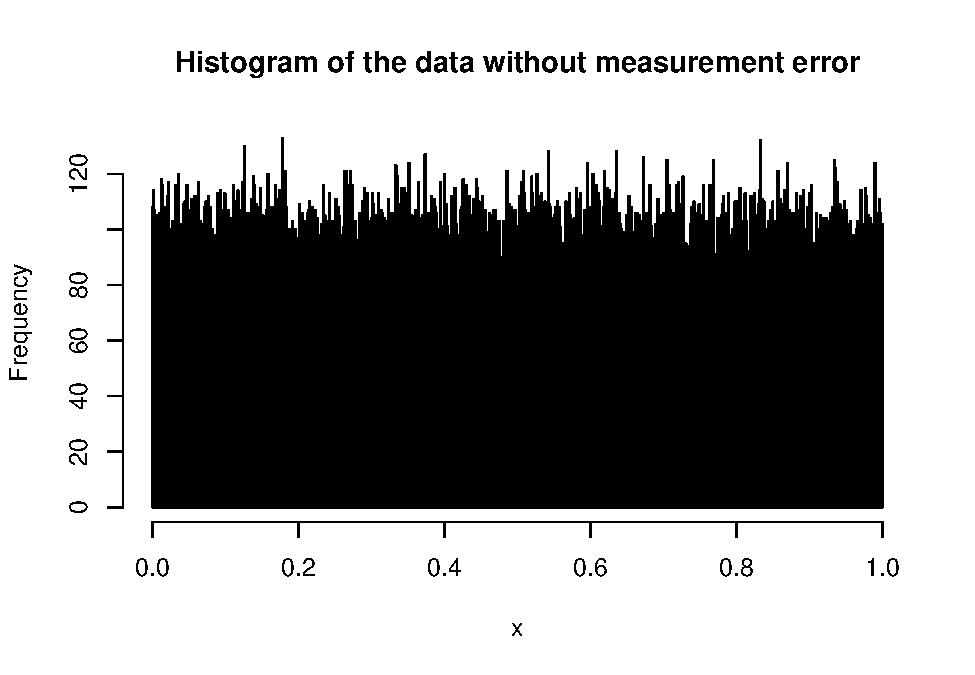
\includegraphics{49045_PB4A7_Report_files/figure-latex/unnamed-chunk-8-1.pdf}

Here are the histograms of the data with measurement error. The plot on
the left is when the data is treated as a continuous variable. The
measurement error makes the last bin at the end of every 20 bins contain
more values than others. The plot on the right is when the data is
treated as a discrete variable. Non-random heaping is invisible since
each value in this histogram has its own bin. The values measured with
error that would be binned together in the continuous histogram are
separated here. This makes the heaping invisible in this plot.

\begin{Shaded}
\begin{Highlighting}[]
\FunctionTok{par}\NormalTok{(}\AttributeTok{mfrow =} \FunctionTok{c}\NormalTok{(}\DecValTok{1}\NormalTok{, }\DecValTok{2}\NormalTok{))}
\FunctionTok{hist}\NormalTok{(x\_error, }\AttributeTok{breaks =} \FunctionTok{seq}\NormalTok{(}\DecValTok{0}\NormalTok{, }\DecValTok{1}\NormalTok{, }\AttributeTok{by =} \FloatTok{0.001}\NormalTok{),}
     \AttributeTok{main =} \StringTok{"Histogram of the data }\SpecialCharTok{\textbackslash{}n}\StringTok{ with measurement error }\SpecialCharTok{\textbackslash{}n}\StringTok{ as a continuous variable"}\NormalTok{)}
\FunctionTok{barplot}\NormalTok{(}\FunctionTok{table}\NormalTok{(x\_discrete), }\AttributeTok{xlab =} \StringTok{"x\_error"}\NormalTok{, }\AttributeTok{ylab =} \StringTok{"Frequency"}\NormalTok{,}
        \AttributeTok{main =} \StringTok{"Histogram of the data }\SpecialCharTok{\textbackslash{}n}\StringTok{ with measurement error }\SpecialCharTok{\textbackslash{}n}\StringTok{ as a discrete variable"}\NormalTok{)}
\end{Highlighting}
\end{Shaded}

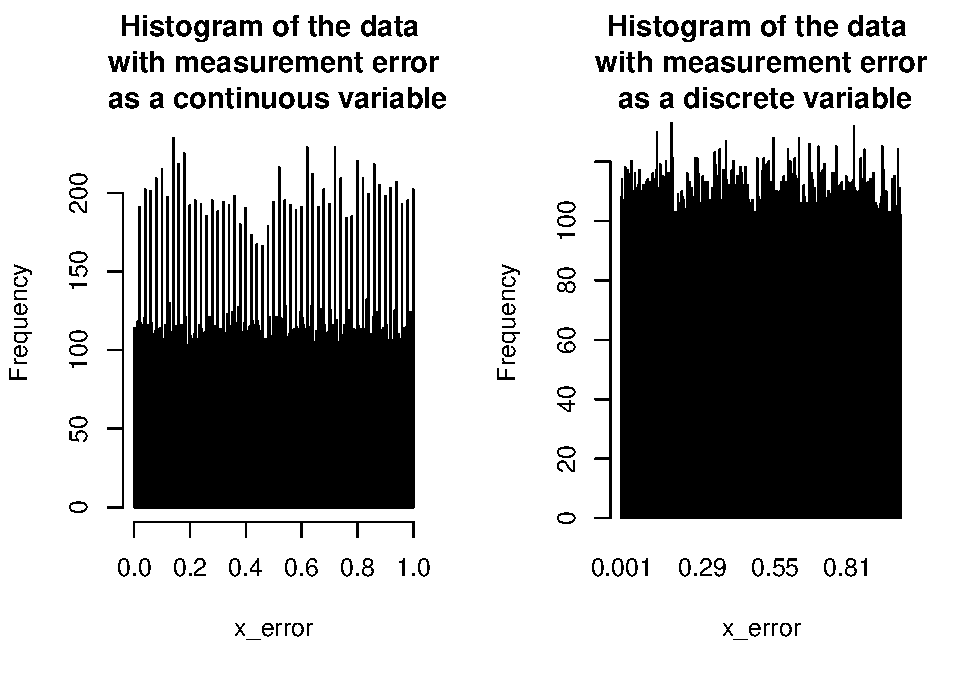
\includegraphics{49045_PB4A7_Report_files/figure-latex/unnamed-chunk-9-1.pdf}

\hypertarget{the-necessity-of-local-polynomials-in-a-donut-hole-model}{%
\subsection*{The necessity of local polynomials in a donut hole
model}\label{the-necessity-of-local-polynomials-in-a-donut-hole-model}}
\addcontentsline{toc}{subsection}{The necessity of local polynomials in
a donut hole model}

This section gives a simulation example to illustrate why local
polynomials are needed in a donut hole design. Particularly, under some
data generating process, getting rid of the data near the threshold can
lead to a drastic difference between the estimates given by a linear and
a quadratic model.

First generating the data we want.

\begin{Shaded}
\begin{Highlighting}[]
\CommentTok{\# set seed}
\FunctionTok{set.seed}\NormalTok{(}\DecValTok{34827}\NormalTok{)}

\DocumentationTok{\#\# simulate the data \#\#}
\CommentTok{\# generate the running variable}
\NormalTok{n }\OtherTok{\textless{}{-}} \DecValTok{100}
\NormalTok{x }\OtherTok{\textless{}{-}} \FunctionTok{seq}\NormalTok{(}\SpecialCharTok{{-}}\FloatTok{0.5}\NormalTok{, }\FloatTok{0.5}\NormalTok{, }\AttributeTok{length.out =}\NormalTok{ n)}
\NormalTok{x\_sq }\OtherTok{\textless{}{-}}\NormalTok{ x}\SpecialCharTok{\^{}}\DecValTok{2}
\CommentTok{\# generate the indicator variable, setting 0 as the cutoff point}
\NormalTok{ind }\OtherTok{\textless{}{-}} \FunctionTok{ifelse}\NormalTok{(x }\SpecialCharTok{\textless{}} \DecValTok{0}\NormalTok{, }\DecValTok{0}\NormalTok{, }\DecValTok{1}\NormalTok{)}
\CommentTok{\# mean value of the outcome}
\NormalTok{mu\_left }\OtherTok{\textless{}{-}} \DecValTok{1} \SpecialCharTok{+} \FloatTok{0.05}\SpecialCharTok{*}\NormalTok{x[}\FunctionTok{which}\NormalTok{(ind }\SpecialCharTok{==} \DecValTok{0}\NormalTok{)]}
\NormalTok{mu\_right }\OtherTok{\textless{}{-}} \FloatTok{1.1} \SpecialCharTok{{-}} \FloatTok{0.02}\SpecialCharTok{*}\NormalTok{x[}\FunctionTok{which}\NormalTok{(ind }\SpecialCharTok{==} \DecValTok{1}\NormalTok{)] }\SpecialCharTok{+}\NormalTok{ x[}\FunctionTok{which}\NormalTok{(ind }\SpecialCharTok{==} \DecValTok{1}\NormalTok{)]}\SpecialCharTok{\^{}}\DecValTok{2}
\NormalTok{mu }\OtherTok{\textless{}{-}} \FunctionTok{c}\NormalTok{(mu\_left, mu\_right)}
\CommentTok{\# simulate outcome variable with random error \textasciitilde{} norm(0, 0.02)}
\NormalTok{y }\OtherTok{\textless{}{-}} \FunctionTok{rnorm}\NormalTok{(n, mu, }\FloatTok{0.02}\NormalTok{)}
\end{Highlighting}
\end{Shaded}

Here are the estimates given by the regular RDD models. We can see the
linear and the quadratic models are already giving different estimates.

\begin{Shaded}
\begin{Highlighting}[]
\DocumentationTok{\#\# regular RDD \#\#}
\CommentTok{\# linear model}
\NormalTok{model\_linear }\OtherTok{\textless{}{-}} \FunctionTok{lm}\NormalTok{(y }\SpecialCharTok{\textasciitilde{}}\NormalTok{ ind}\SpecialCharTok{*}\NormalTok{x)}
\FunctionTok{summary}\NormalTok{(model\_linear)}
\end{Highlighting}
\end{Shaded}

\begin{verbatim}
## 
## Call:
## lm(formula = y ~ ind * x)
## 
## Residuals:
##       Min        1Q    Median        3Q       Max 
## -0.066646 -0.015409 -0.002732  0.012278  0.056368 
## 
## Coefficients:
##             Estimate Std. Error t value Pr(>|t|)    
## (Intercept) 1.003208   0.006792 147.713  < 2e-16 ***
## ind         0.046232   0.009605   4.813 5.52e-06 ***
## x           0.056133   0.023293   2.410   0.0179 *  
## ind:x       0.456895   0.032941  13.870  < 2e-16 ***
## ---
## Signif. codes:  0 '***' 0.001 '**' 0.01 '*' 0.05 '.' 0.1 ' ' 1
## 
## Residual standard error: 0.02401 on 96 degrees of freedom
## Multiple R-squared:  0.9554, Adjusted R-squared:  0.954 
## F-statistic: 685.3 on 3 and 96 DF,  p-value: < 2.2e-16
\end{verbatim}

\begin{Shaded}
\begin{Highlighting}[]
\CommentTok{\# quadratic model}
\NormalTok{model\_qua }\OtherTok{\textless{}{-}} \FunctionTok{lm}\NormalTok{(y }\SpecialCharTok{\textasciitilde{}}\NormalTok{ ind}\SpecialCharTok{*}\NormalTok{(x }\SpecialCharTok{+}\NormalTok{ x\_sq))}
\FunctionTok{summary}\NormalTok{(model\_qua)}
\end{Highlighting}
\end{Shaded}

\begin{verbatim}
## 
## Call:
## lm(formula = y ~ ind * (x + x_sq))
## 
## Residuals:
##       Min        1Q    Median        3Q       Max 
## -0.049210 -0.013100 -0.000029  0.012250  0.049643 
## 
## Coefficients:
##              Estimate Std. Error t value Pr(>|t|)    
## (Intercept)  1.002073   0.008416 119.061  < 2e-16 ***
## ind          0.090294   0.011903   7.586 2.34e-11 ***
## x            0.042659   0.076987   0.554    0.581    
## x_sq        -0.026679   0.147601  -0.181    0.857    
## ind:x       -0.039505   0.108876  -0.363    0.718    
## ind:x_sq     1.036230   0.208739   4.964 3.07e-06 ***
## ---
## Signif. codes:  0 '***' 0.001 '**' 0.01 '*' 0.05 '.' 0.1 ' ' 1
## 
## Residual standard error: 0.01982 on 94 degrees of freedom
## Multiple R-squared:  0.9702, Adjusted R-squared:  0.9686 
## F-statistic: 612.5 on 5 and 94 DF,  p-value: < 2.2e-16
\end{verbatim}

We now run the donut hole models with the data points in the window
\([-0.1, 0.1]\) dropped. We can see the difference between the two
models gets even bigger.

\begin{Shaded}
\begin{Highlighting}[]
\DocumentationTok{\#\# donut whole RDD \#\#}
\CommentTok{\# create an index for the data to be removed }
\CommentTok{\# here the data within the window [{-}0.1, 0.1] are dropped}
\NormalTok{index }\OtherTok{\textless{}{-}} \FunctionTok{which}\NormalTok{(}\FunctionTok{abs}\NormalTok{(x) }\SpecialCharTok{\textless{}=} \FloatTok{0.1}\NormalTok{)}
\NormalTok{x\_donut }\OtherTok{\textless{}{-}}\NormalTok{ x[}\SpecialCharTok{{-}}\NormalTok{index]}
\NormalTok{x\_sq\_donut }\OtherTok{\textless{}{-}}\NormalTok{ x\_sq[}\SpecialCharTok{{-}}\NormalTok{index]}
\NormalTok{ind\_donut }\OtherTok{\textless{}{-}}\NormalTok{ ind[}\SpecialCharTok{{-}}\NormalTok{index]}
\NormalTok{y\_donut }\OtherTok{\textless{}{-}}\NormalTok{ y[}\SpecialCharTok{{-}}\NormalTok{index]}

\CommentTok{\# linear model}
\NormalTok{donut\_linear }\OtherTok{\textless{}{-}} \FunctionTok{lm}\NormalTok{(y\_donut }\SpecialCharTok{\textasciitilde{}}\NormalTok{ ind\_donut}\SpecialCharTok{*}\NormalTok{x\_donut)}
\FunctionTok{summary}\NormalTok{(donut\_linear)}
\end{Highlighting}
\end{Shaded}

\begin{verbatim}
## 
## Call:
## lm(formula = y_donut ~ ind_donut * x_donut)
## 
## Residuals:
##       Min        1Q    Median        3Q       Max 
## -0.059963 -0.012245  0.000161  0.013934  0.052182 
## 
## Coefficients:
##                   Estimate Std. Error t value Pr(>|t|)    
## (Intercept)       0.997372   0.009385 106.277   <2e-16 ***
## ind_donut         0.010642   0.013272   0.802    0.425    
## x_donut           0.040351   0.028904   1.396    0.167    
## ind_donut:x_donut 0.589272   0.040876  14.416   <2e-16 ***
## ---
## Signif. codes:  0 '***' 0.001 '**' 0.01 '*' 0.05 '.' 0.1 ' ' 1
## 
## Residual standard error: 0.02131 on 76 degrees of freedom
## Multiple R-squared:  0.9703, Adjusted R-squared:  0.9692 
## F-statistic: 828.7 on 3 and 76 DF,  p-value: < 2.2e-16
\end{verbatim}

\begin{Shaded}
\begin{Highlighting}[]
\CommentTok{\# quadratic model}
\NormalTok{donut\_qua }\OtherTok{\textless{}{-}} \FunctionTok{lm}\NormalTok{(y\_donut }\SpecialCharTok{\textasciitilde{}}\NormalTok{ ind\_donut}\SpecialCharTok{*}\NormalTok{(x\_donut }\SpecialCharTok{+}\NormalTok{ x\_sq\_donut))}
\FunctionTok{summary}\NormalTok{(donut\_qua)}
\end{Highlighting}
\end{Shaded}

\begin{verbatim}
## 
## Call:
## lm(formula = y_donut ~ ind_donut * (x_donut + x_sq_donut))
## 
## Residuals:
##       Min        1Q    Median        3Q       Max 
## -0.051596 -0.012810  0.000166  0.009101  0.052266 
## 
## Coefficients:
##                      Estimate Std. Error t value Pr(>|t|)    
## (Intercept)           0.97677    0.02237  43.666  < 2e-16 ***
## ind_donut             0.09586    0.03163   3.030  0.00336 ** 
## x_donut              -0.11927    0.16139  -0.739  0.46224    
## x_sq_donut           -0.26337    0.26244  -1.004  0.31888    
## ind_donut:x_donut     0.24830    0.22824   1.088  0.28017    
## ind_donut:x_sq_donut  1.08934    0.37115   2.935  0.00444 ** 
## ---
## Signif. codes:  0 '***' 0.001 '**' 0.01 '*' 0.05 '.' 0.1 ' ' 1
## 
## Residual standard error: 0.02017 on 74 degrees of freedom
## Multiple R-squared:  0.9741, Adjusted R-squared:  0.9724 
## F-statistic: 557.7 on 5 and 74 DF,  p-value: < 2.2e-16
\end{verbatim}

The moral here is essentially that removing data points may influence
the conclusions we draw when comparing models with different functional
forms. Even if the results may be robust to different functional forms
under the regular RDD design, they can still be sensitive to the
functional assumption under the donut hole design. It is thus a good
idea to use both linear models and polynomials in the donut hole design.

\end{document}
